\documentclass[]{report}
\usepackage[hmargin=1.25in,vmargin=1in]{geometry} %调整页边距
% \usepackage[inner=1in,outer=1.25in]{geometry} %书籍左右不等宽排版
\usepackage[utf8]{inputenc}
\usepackage[]{ctex} %据说可以直接调用诸如 \kaishu \fangsong \heiti 的命令修改字体
\usepackage[svgnames]{xcolor} % Using colors
% \usepackage{background} % To include background images
\usepackage{fancyhdr} % Needed to define custom headers/footers
\usepackage[]{xeCJK}
\setCJKmainfont[BoldFont = STHeiti, ItalicFont = STKaiti]{Songti SC Light} %中文主字体
\setCJKsansfont[BoldFont = Weibei SC, ItalicFont = HanziPen SC]{Xingkai SC Light} %中文无衬线字体
\setCJKmonofont[BoldFont = Libian SC, ItalicFont = STFangsong]{Yuanti SC Light} %中文等宽字体
\setmainfont{Times New Roman} %\rmfamily
\setsansfont[ItalicFont = American Typewriter]{Comic Sans MS} %\sffamily
\setmonofont{Courier} %\ttfamily
\newfontfamily\monaco{Courier} % 用于代码段字体设置
\usepackage{titlesec}
\titleformat{\chapter}{\centering\huge\bfseries}{第~\thechapter~章}{1em}{}
\titleformat{\section}{\Large\bfseries}{第~\thesection~节}{1em}{}
\usepackage{lipsum} %填充文本

\usepackage{ulem} %解决下划线、删除线之类的
\usepackage{listings}
\lstset{
language=C++,
numberstyle = \monaco,
basicstyle = \monaco,
keywordstyle = \color{blue}\bfseries,
commentstyle=\color[HTML]{006400},
tabsize = 4,
%backgroundcolor=\color{bg}
emph = {int,float,double,char},emphstyle=\color{cyan},
emph = {[2]const, typedef},emphstyle = {[2]\color{red}} }

\makeatletter
\newif\if@restonecol
\makeatother
\let\algorithm\relax
\let\endalgorithm\relax
\usepackage[linesnumbered,ruled,vlined]{algorithm2e}%[ruled,vlined]{
\usepackage{algpseudocode}
\usepackage{amsmath}
\renewcommand{\algorithmicrequire}{\textbf{Input:}}  % Use Input in the format of Algorithm
\renewcommand{\algorithmicensure}{\textbf{Output:}} % Use Output in the format of Algorithm

\usepackage{amsmath} %数学公式问题
\usepackage{amsthm} %公式环境,如proof
\usepackage{booktabs} %三线表
\newcommand{\tabincell}[2]{\begin{tabular}{@{}#1@{}}#2\end{tabular}} %解决单元格内部换行的问题
% 比如这个 Beijing & 0,5 & 1,6 & 2,7 & 3,8 & 4,9 & The number changes every 3 months \\
% 改成这个 \tabincell{l}{Beijing}& \tabincell{c}{0,5}& \tabincell{c}{1,6}& \tabincell{c}{2,7}& \tabincell{c}{3,8}& \tabincell{c}{4,9}& \tabincell{c}{The number changes \\ every 3 months} \\
% 一个单元格过长,整行都需要修改
% 可以配合 \resizebox*{h-width}{v-width}{contents, e.g.tabular} 使用

\usepackage{mathrsfs} %在公式里面使用那个最花的字体
\usepackage{amssymb} %公式里面用空心黑体和旧式字体
\usepackage{amssymb} %AMS符号
\usepackage{amsthm} %AMS定理环境

\usepackage{markdown} %使用markdown语法,在编译时需要打开 shell-escape 标记,即 $ xelatex --shell-escape example.tex
\markdownSetup{hashEnumerators = true} %允许使用 #. 的方式编写有序列表
\markdownSetup{inlineFootnotes = true} %允许使用脚注形式的超链接,调用语法为 [anchor](uri), ^[footnote], <uri>
\markdownSetup{fencedCode = true} %以反引号和缩进来插入代码段,相当于 verbatim
\markdownSetup{
  pipeTables = true
} %支持表格的用法 (图片已经在markdown包里面支持了)
% \usepackage{booktabs} %解决三线表的线条粗细问题

\usepackage{graphicx} %插入图片
\usepackage{pdfpages} %插入PDF文件
\usepackage{makeidx}

\usepackage{tikz} %带圈字符
\usepackage{etoolbox} %带圈字符 (提供robustify)
\usepackage{enumitem}
\newcommand*{\circled}[1]{\lower.7ex\hbox{\tikz\draw (0pt, 0pt)%
    circle (.5em) node {\makebox[1em][c]{\small #1}};}} %新定义命令:带圈字符
\robustify{\circled}
% \usepackage{enumerate} %有序列表

\usepackage{hyperref} %超链接
% \usepackage[hidelinks]{hyperref} %隐藏超链接的红框
\markdownSetup{
  inlineFootnotes = true,
  renderers = {
    link = {\href{#3}{#1}},
  }
} % markdown块中使用直接点进去的超链接
% \setlist[enumerate,1]{label=(\arabic*).,font=\textup,leftmargin=7mm,labelsep=1.5mm,topsep=0mm,itemsep=-0.8mm}
% \setlist[enumerate,2]{label=(\alph*).,font=\textup,leftmargin=7mm,labelsep=1.5mm,topsep=-0.8mm,itemsep=-0.8mm}

\usepackage{braket}

%%%%%% Setting up the style

% \setlength\parindent{0pt} % Gets rid of all indentation
% \backgroundsetup{contents={\includegraphics[width=\textwidth]{ustc-name.pdf}},scale=0.4,placement=top,opacity=0.6,color=cyan,vshift=-20pt} %  USTC Logo

\pagestyle{fancy} % Enables the custom headers/footers

% 使用默认的Chapter页眉
% \lhead{} \rhead{} % Headers - all  empty

% \title{\vspace{-1.8cm}  \color{DarkRed} Laboratory Rotation Report}
% \subtitle{Title of the proposal % Title of the rotation project
% \vspace{-2cm} }
% \date{\today} % No date

\lfoot{\color{Grey} \textit{上官凝}}  % Write your name here
\rfoot{ \color{Grey} 编译原理 }
\cfoot{\color{Grey} \thepage}

\renewcommand{\headrulewidth}{0.0pt} % No header rule
\renewcommand{\footrulewidth}{0.4pt} % Thin footer rule

\title{{\huge {编译原理笔记}}}
\author{上官凝}
\date{\today}

\linespread{1.3} %行间距为1.3倍默认间距 (1.3 x 1.2倍字符宽度)

\makeindex

\begin{document}
\theoremstyle{definition} \newtheorem{theorem}{Thm}[section] %定义一个定理Thm,序号为section的下一级序号
\theoremstyle{definition} \newtheorem{definition}{Def}[section] %定义一个定义Def,序号为section的下一级序号
\theoremstyle{plain} \newtheorem{lemma}{lemma}[section] %引理

	\maketitle
	\newpage

	\tableofcontents
	\newpage

	\chapter{词法分析}
	\begin{figure}
		\centering
		\begin{minipage}{40em}
			\centering
			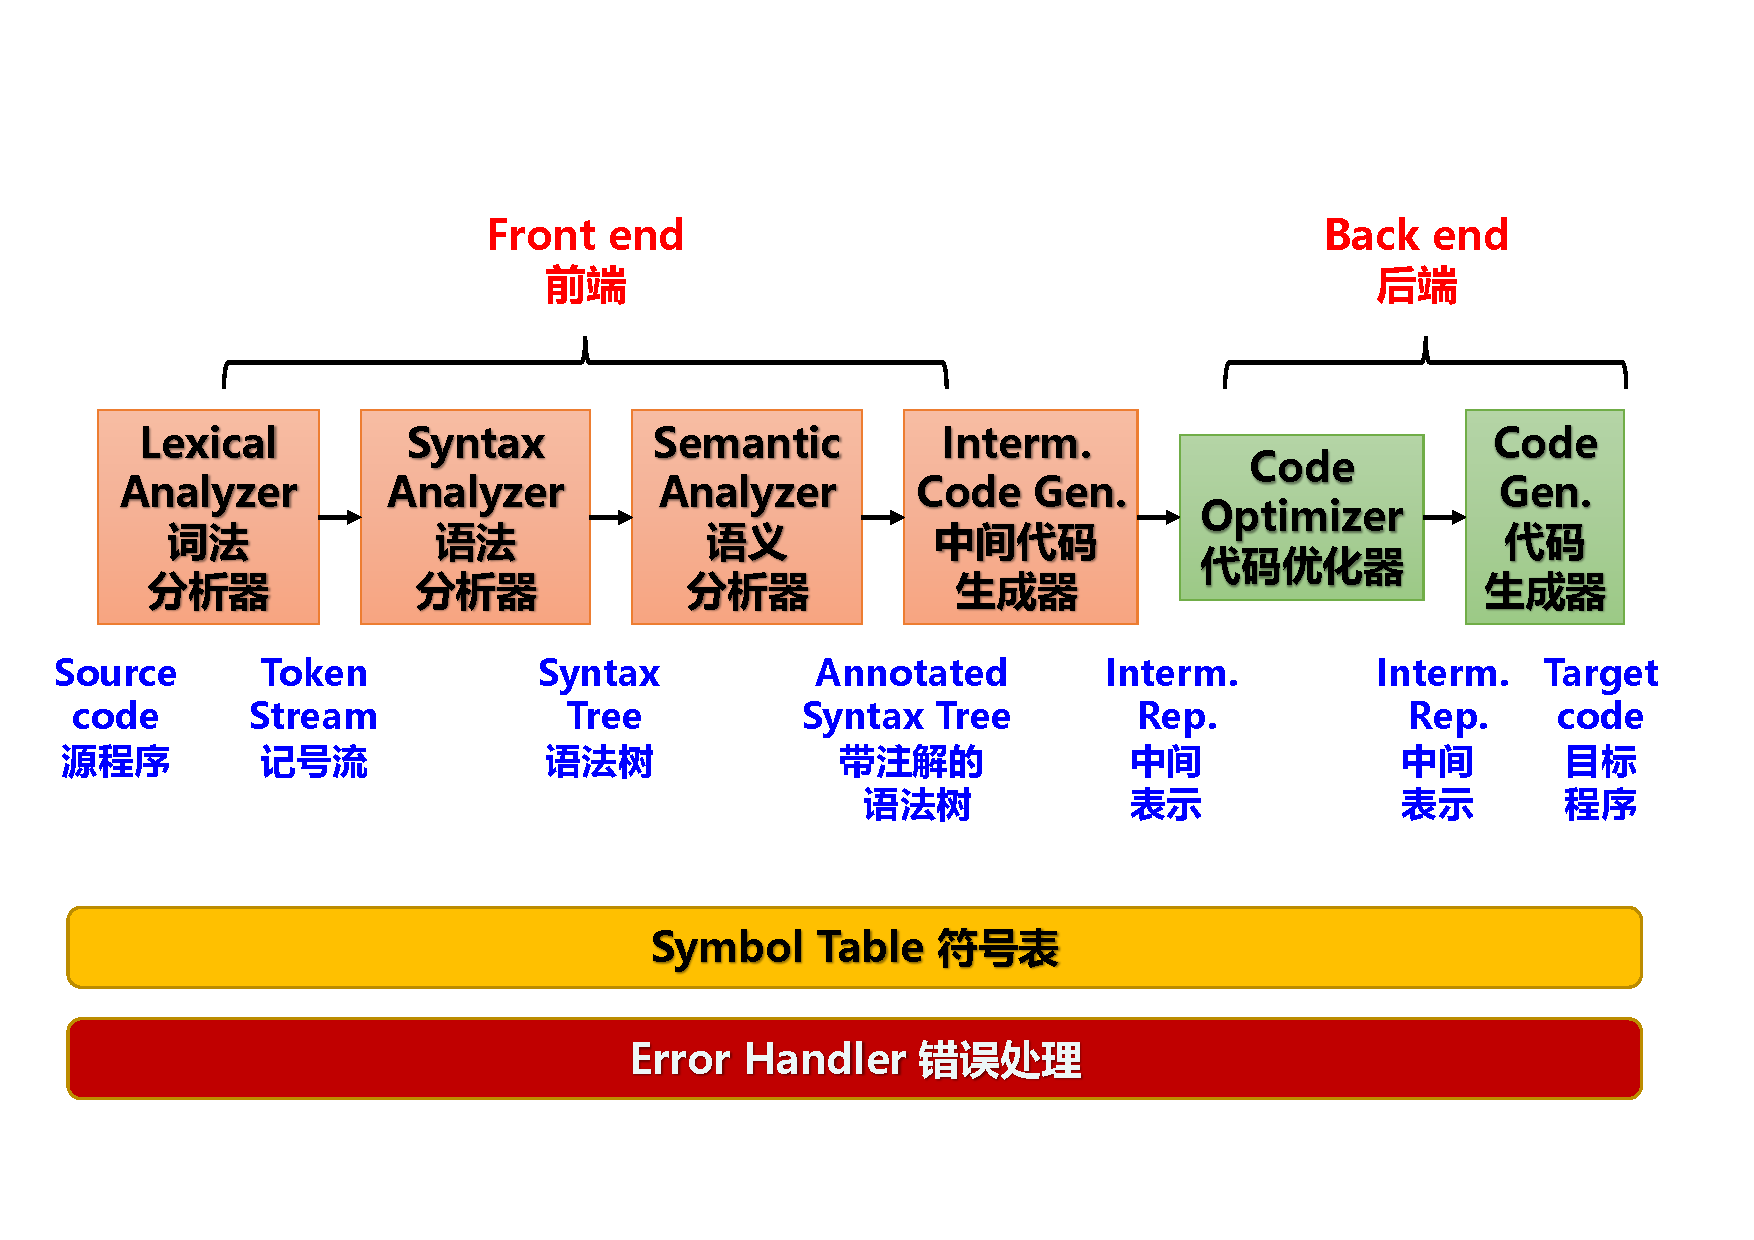
\includegraphics[scale = 0.3]{images/lecture_intro.pdf}
			\caption{编译器总览}
		\end{minipage}
	\end{figure}
	词法分析器的任务是把构成源程序的字符流翻译成词法记号流。其目的是将输入字符串识别为有意义的子串
	\begin{enumerate}
		\item 子串的种类(Name)
		\item 可帮助解释和理解该子串的属性(Attribute)
		\item 可描述具有相同特征的子串的模式(Pattern)
	\end{enumerate}
	\section{词法记号及属性、描述和识别}
		\subsection{词法记号和属性}
		词法记号由记号名和可选的属性值构成的二元组,经常使用记号名来引用记号。一个记号的模式描述属于该记号的词法单元的形式。词法单元是源程序中匹配一个记号模式的字符序列,它由词法分析器识别为该记号的一个实例。\textit{为什么需要属性?}概括的说,记号名影响语法分析的决策,属性影响记号的翻译。
		\subsection{串和语言}
		语言表示字母表上的一个串集,属于该语言的串称为该语言的句子或字,注意$\varnothing$和$\{\varepsilon\}$这样的抽象语言也符合这个定义。其运算参考字符串的运算(连接)和集合的运算(交并补etc)
		\subsection{正则表达式}
		约定:
		\begin{enumerate}
			\item 闭包运算($^*$)有最高的优先级并且是左结合的运算
			\item 连接运算(两个正规式并列)的优先级次之且也是左结合的运算
			\item 选择运算($\mid$)的优先级最低并且也是左结合的运算
			\item 零个或一个实例($r?$)表示 $r\mid\varepsilon$
			\item 字符组($[abc]$)表示$a\mid b\mid c$
			\item 缩写字符组($[a-z]$)表示$a\mid b\mid\cdots\mid z$
		\end{enumerate}\par
		可以对正规式命名,并用这些名字来引用相应的正规式。可以采用自底向上的方式来构建正规定义
		\subsection{状态转换图}
		(打个广告:在我的\href{http://home.ustc.edu.cn/~astark/}{主页}上面放了一个在线画FSM的网址连接)\par
		大概长这样(这个是分析各种运算符以及注释的一个转换图,数字识别没有画完整)(IN是指intermediate,中间态):\par
		\begin{figure}[h!]
			\centering
			\begin{minipage}{40em}
				\centering
				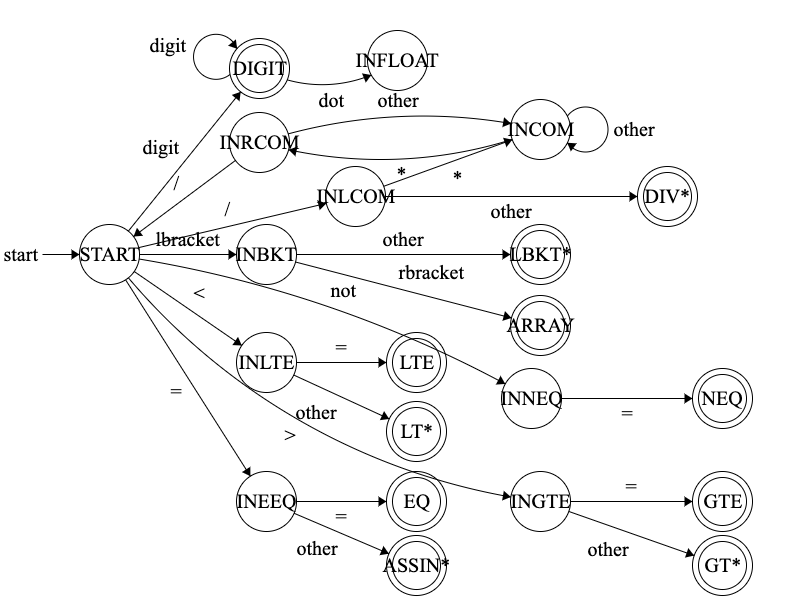
\includegraphics[scale = 0.35]{images/FSM_Sample.png}
			\end{minipage}
		\end{figure}\par
		在词法分析时,会出现“移进归约冲突”(这里不是这么叫的,我只是借鉴一下这种说法)。就是识别到一个token,它可能是一个关键字,也有可能是其他token的前缀。这时候应用最长匹配规则,即lookahead,如果不符合词法规则(状态机无法跳转)就回退。\par
		值得注意的是,词法分析器对程序采取非常局部的观点,即词法分析器只会管给定的程序(一个字符串)是不是能拆分成符合词法定义的token流。这些token在词法分析器看来是相互无关的。
		\subsection{关于FLEX的正则表达式}
		众所周知,实验会用到FLEX,在写\verb|.l|文件的时候要写正则表达式,大概规则如下:
		\begin{enumerate}
			\item \verb|.| 匹配任何单个字符,除 \verb|\n|.
			\item \verb|-| 表示匹配范围,如:\verb|a-z|,表示匹配a-z之间的任何字符
			\item \verb|*| 匹配前面表达式的零个或多个拷贝。
			\item \verb|[]| 匹配括号内的任意字符的字符类,第一个符号是 \verb|^|,表示匹配除括号中的字符以外的任意字符,如 \verb|[^/]| 表示除斜杠以外的所有字符。
			\item \verb|()| 表示里面的模式被允许匹配多少次。
			\item \verb|\| 用于转义字符
			\item \verb|+| 匹配前面表达式一次或多次出现。
			\item \verb|?| 匹配前面表达式零次或1次出现。
			\item \verb||| 匹配前面表达式或随后表达式
			\item \verb|""| 引号中的每个字符解释为字面意思
			\item \verb|{}| 指示一个模式可能出现的次数,后面可以跟 \verb|*| 或者 \verb|+|
		\end{enumerate}\par
		以及,可以\textbf{参考}\href{https://blog.csdn.net/u014594922/article/details/51224231}{这个}文章
	\section{有限自动机}
		\subsection{NFA和DFA}
		NFA(不确定的有限自动机)可以把同样的符号标记在出自同一个状态的多条边上,而DFA(确定的有限自动机)是NFA的特殊情况,其中:任何状态下都没有$\varepsilon$转换;且对任何状态s和任何输入符号a,最多只能有一条表示为a的边离开s
		\subsection{正则表达式到NFA}
		基本模型有$a\mid b$、$ab$、$s^*$和$(s)$,分别对应以下的图:
		\begin{figure}[h!]
			\centering
			\begin{minipage}{40em}
				\begin{minipage}{18em}
					\centering
					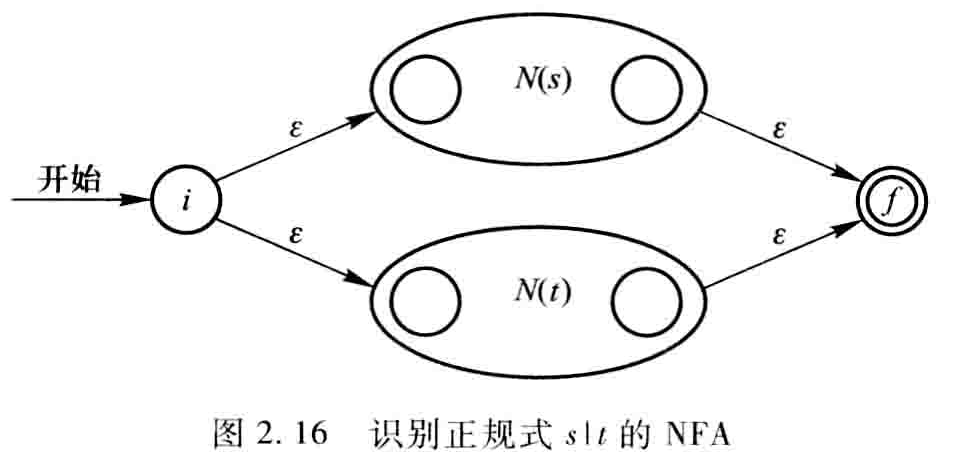
\includegraphics[scale = 0.18]{images/s_mid_t.png}
				\end{minipage}
				\begin{minipage}{18em}
					\centering
					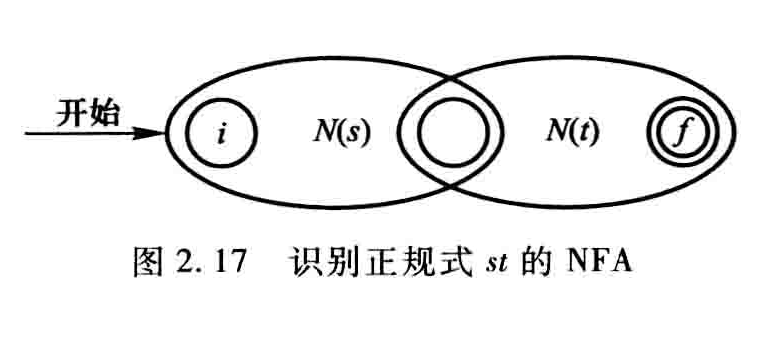
\includegraphics[scale = 0.23]{images/st.png}
				\end{minipage}
			\end{minipage}
		\end{figure}
		\begin{figure}[ht!]
			\centering
			\begin{minipage}{30em}
				\centering
				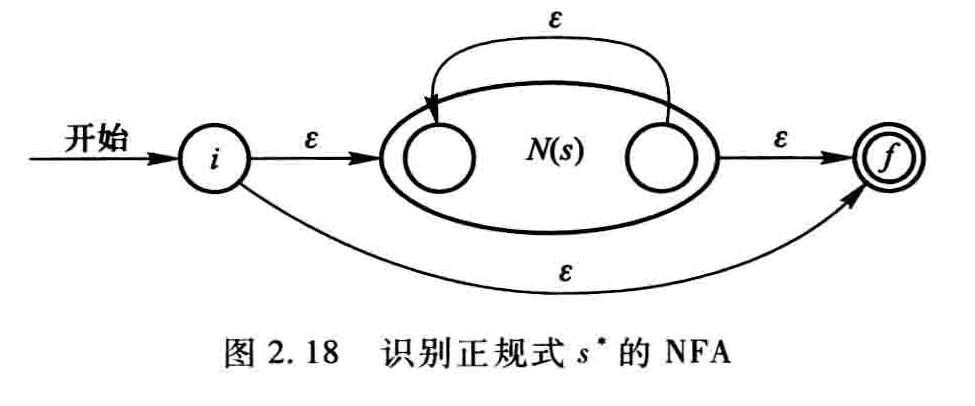
\includegraphics[scale = 0.25]{images/s_star.png}
			\end{minipage}
		\end{figure}
		\subsection{NFA到DFA}
		NFA的状态是DFA的状态集合(闭包)。主要的有两步:
		\begin{enumerate}
			\item 递归计算出来包含状态0(start状态)的闭包(就是经过$\varepsilon$能到达的所有状态)
			\item 这个闭包在接收某个输入之后可能到达的新的状态闭包
		\end{enumerate}\par
		然后对新的闭包迭代第二步,直到没有新的了
		\subsection{DFA的化简}
		观察DFA的状态转换表,将对于任意输入符号,其跳转都一样的几个状态合并为同一状态,并选取一个代表。首先要\textbf{分开接受状态和非接受状态}


	\chapter{语法分析}
	\textit{输入:词法分析获得的记号序列;输出:程序的语法树}。需要一种可以描述合法记号序列的语言、一种可以区分合法和非法的记号序列的方法。正则表达式不能用于描述配对或嵌套的结构,这是因为有限自动机不能记录重复访问同一状态的次数。\par
	\section{上下文无关文法}
		上下文无关文法CFG是由一个四元组$(V_T,V_N,S,P)$组成的:
		\begin{enumerate}
			\item 终结符:就是“句型”最终需要化成的形式,里面的元素都是确定的符号,也称为$token$。\textit{在谈论编程语言的文法时,记号名时终结符的同义词。}
			\item 非终结符:可以认为是推导过程中的“中间变量”,或“形式参量”,用自下而上的角度来说,非终结符是终结符或/和非终结符的规约
			\item 开始符号:是语法树的$root$
			\item 产生式的有限集合:生成规则,用$\to$
		\end{enumerate}
		\subsection{CFG推导}
		CFG推导是“从文法推出文法所描述的语言中所包含的合法串集合的动作”,也就是说,从开始符号开始,利用生成规则进行迭代替换,得到句型。“上下文无关”是指在推导过程中,每一步$\alpha A\beta\Rightarrow\alpha\gamma\beta$仅依赖于$A\to\gamma$,而与$\alpha,\beta$无关。对于语言、文法、句型、句子,语言是句子的集合,句子是实例。最左推导$\Rightarrow_{lm}$和最右推导(规范推导)$\Rightarrow_{rm}$。一步推导$\Rightarrow$和零步或多步推导$\Rightarrow^*$以及一步或多步推导$\Rightarrow^+$。\par
		\subsection{文法的二义性}
		文法的某些句子存在不止一种最左(最右)推导,或者不止一棵分析树,则该文法是二义的。一般是由优先级和结合性的不确定导致的。所以可以通过定义优先级(将多个选项拆分为不同非终结符的嵌套推导规则来认为定义等级划分)来解决这个问题。这样,更接近于开始符号的非终结符就不能直接推导到终结符,更接近于终结符的不能从开始符号终结推导。\textit{左推导优先级从高到低,右推导相反}比如将第一个式子换成下面的几个:
		\[\begin{gathered}
			E\to E+E\mid E*E\mid(E)\mid\mathbf{id}\\
			E\to E+E\mid F\\
			F\to F*F\mid G\\
			G\to (G)\mid\mathbf{id}
		\end{gathered}\]
		\subsection{悬空else文法}
		悬空else文法是一个经典的例子:
		\begin{figure}[h!]
			\centering
			\begin{minipage}{20em}
				\centering
				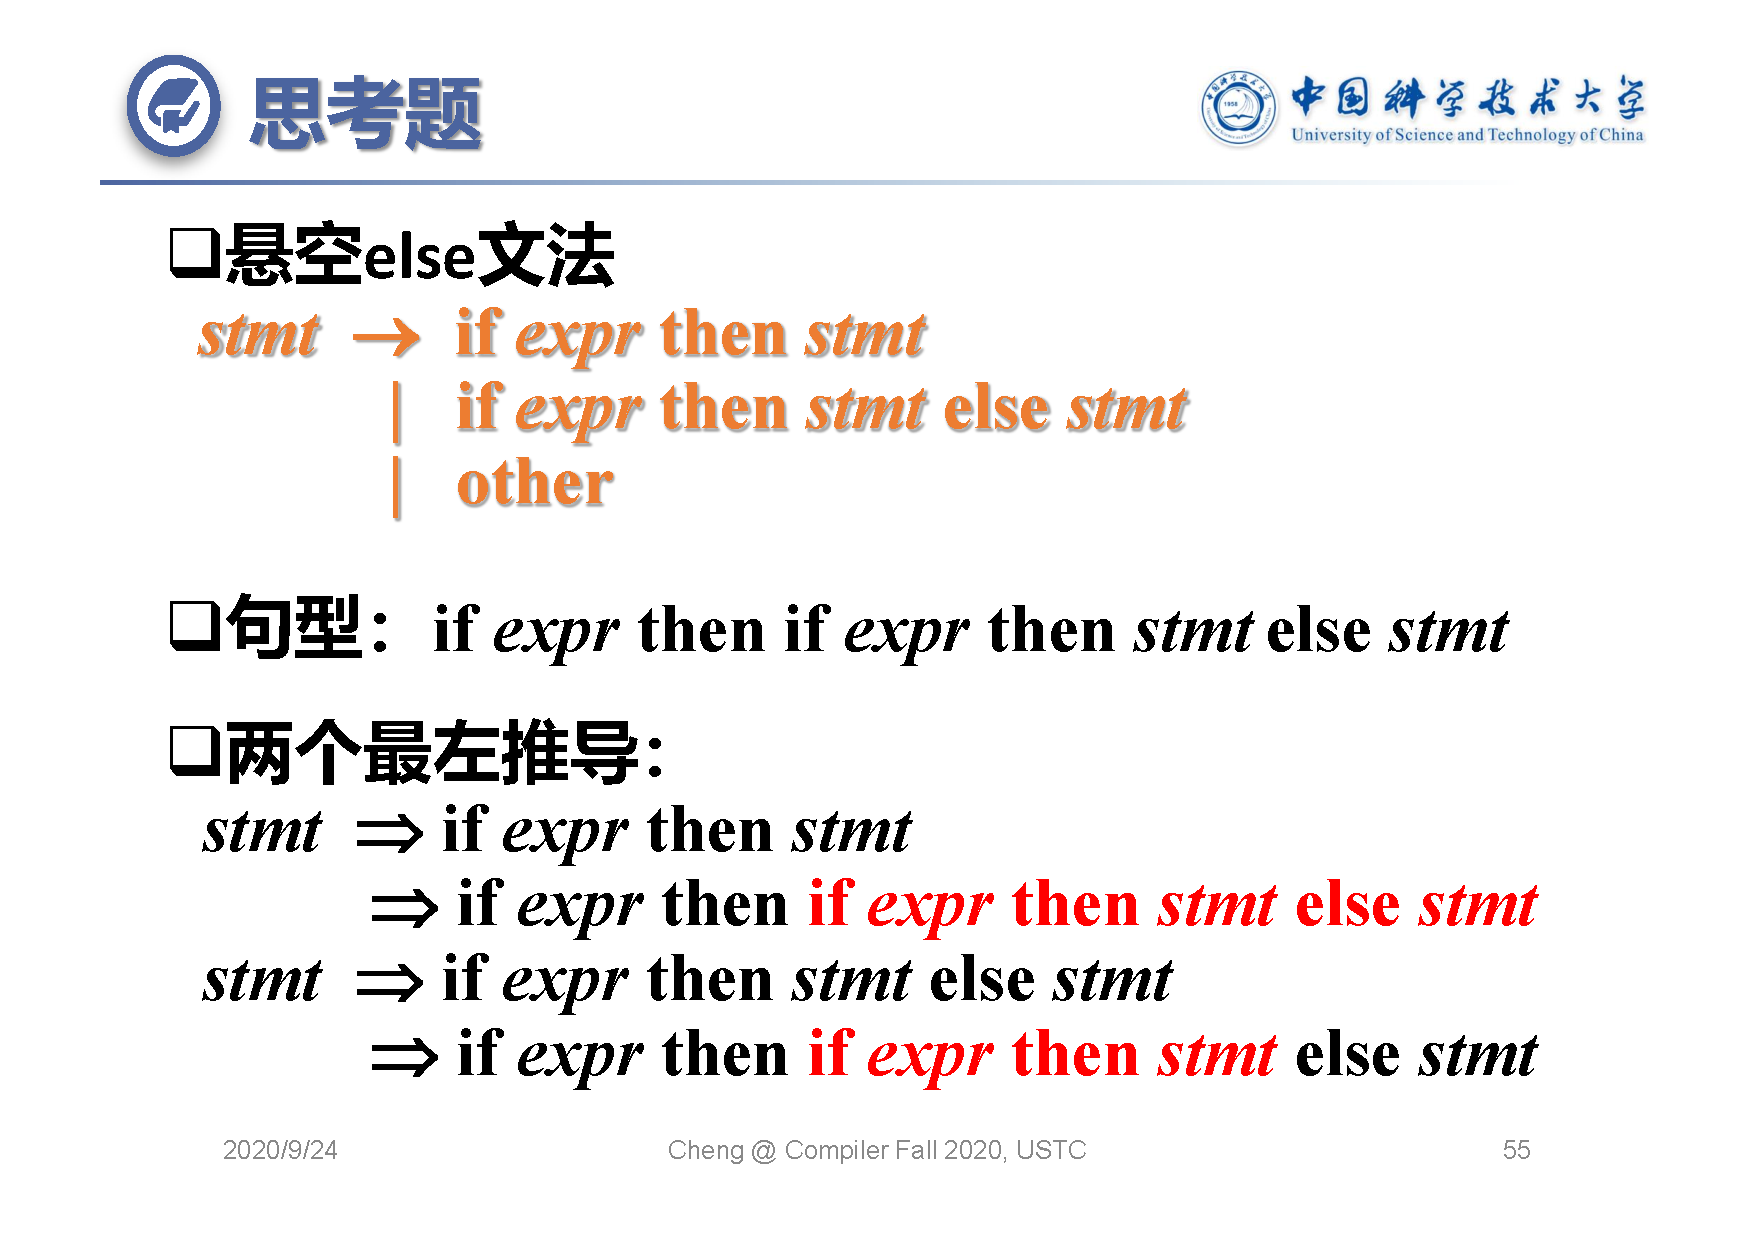
\includegraphics[scale = 0.2]{images/Impending_ELSE.pdf}
				\caption{悬空else文法及其二义性}
			\end{minipage}\quad
			\begin{minipage}{20em}
				\centering
				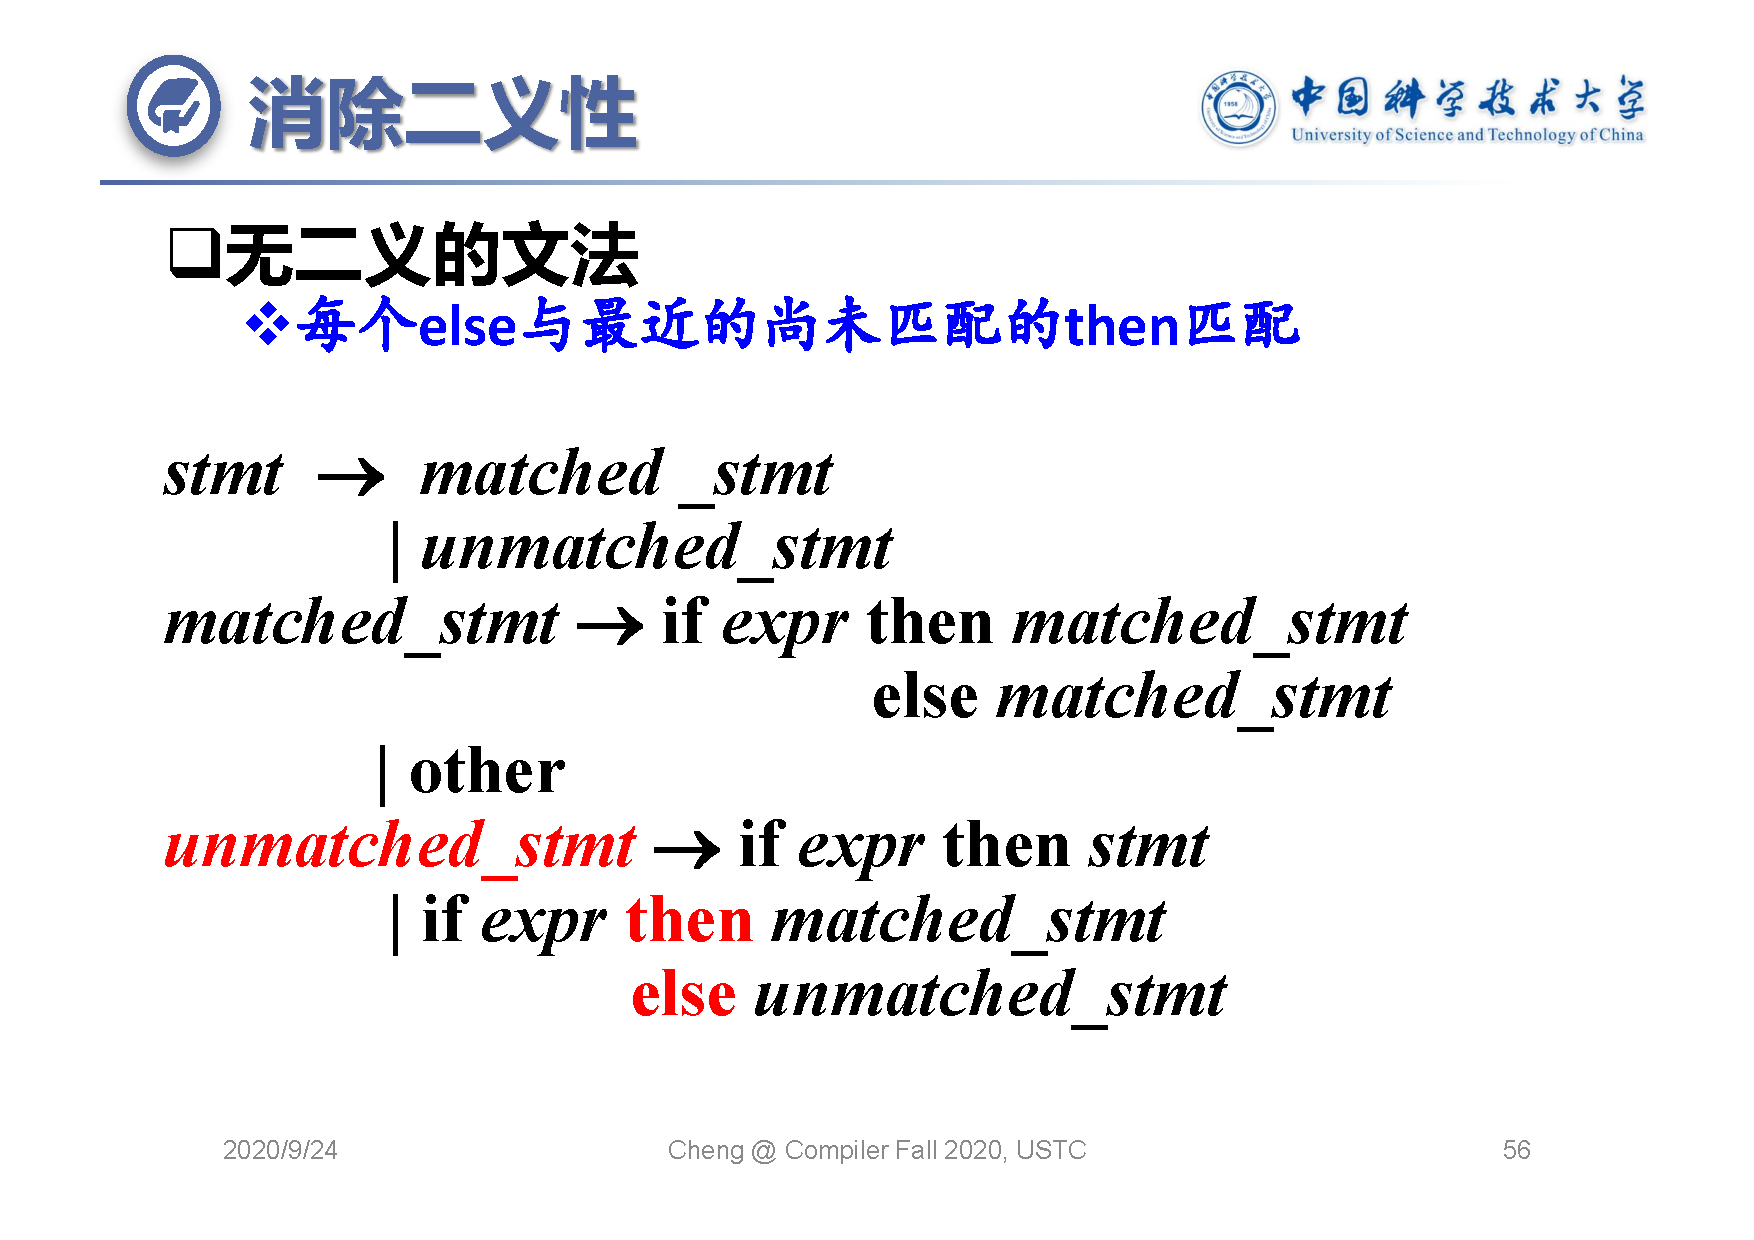
\includegraphics[scale = 0.2]{images/Eliminate_Ambiguity_of_ELSE.pdf}
				\caption{悬空else文法二义性的消除}
			\end{minipage}
		\end{figure}\par
		应当注意的是,文法的二义性并不意味着语言是二义的。只有当产生一个语言的所有文法都是二义的时,才称为是二义的。而且也可以构造允许二义文法的分析器,但要附带消除二义性但规则(剪枝回溯)。值得看到的是,定义无二义文法可能会失去简洁性。
		\subsection{左递归}
		一个文法是左递归的,如果他有非终结符A,对于某个串$\alpha$,存在推导$A\Rightarrow^+A\alpha$。自上而下的分析方法不能用于左递归文法。
	\section{自顶向下分析方法}
		\subsection{递归下降分析方法}
		包括一个输入缓冲区和向前看指针lookahead,自左向右扫描输入串;设计一个辅助过程match(),将lookahead指向的位置与产生式迭代生成的终结符进行匹配,如匹配,将lookahead挪到下一个位置。就是对于一个可能的串,从root开始构建一棵语法的生成树。递归下降也有着自己的一些问题,比如可能进入无限循环。下面是递归下降的三个问题,
		\subsection{消除左递归}
		左递归分为直接左递归和间接左递归。直接左递归有形如$A\rightarrow A\alpha$的产生式,间接左递归是通过有限次迭代(类似于证明序列)得到(非直接左递归首先变成直接左递归,然后消除他)。消除左递归的通用方法如下所示:首先将A的产生式组合在一起:
		\[A\to A\alpha_1\mid A\alpha_2\mid\cdots\mid A\alpha_m\mid\beta_1\mid\beta_2\mid\cdots\mid\beta_n\]
		其中$\beta_i$都不以A开始,$\alpha_i$非空,然后用
		\[\begin{gathered}
			A\to\beta_1A'\mid\beta_2A'\mid\cdots\mid\beta_nA'\\
			A'\to\alpha_1A'\mid\alpha_2A'\mid\cdots\mid\alpha_mA'\mid\varepsilon
		\end{gathered}\]
		代替A的产生式。注意后面加上了一个$\varepsilon$,作为一个终结符结束递归
		\subsection{有左因子的文法}
		有左因子的(left-factored)文法形如$A\to\alpha\beta_1\mid\alpha\beta_2$。在自上而下的分析中,当不清楚应该用非终结符$A$的那个选择来替换它时,可以通过重写$A$产生式来推迟这种决定,推迟到看到足够多的输入,能帮助正确决定所需选择为止。如上式等价于\[\begin{gathered}
			A\to\alpha A'\\
			A\to\beta_1\mid\beta_2
		\end{gathered}\]
		需要注意的是,提取左因子的重写并不能解决二义性,比如之前提到的悬空else文法,提取左因子之后成为
		\[\begin{gathered}
			stmt\to\mathbf{if}\ expr\ \mathbf{then}\ stmt\ optional_else_part\mid\mathbf{other}\\
			optional_else_part\to\mathbf{else}\ stmt\mid\varepsilon
		\end{gathered}\]
		这个文法对于如$\mathbf{if}\ expr\ \mathbf{then}\ \mathbf{if}\ expr\ \mathbf{then}\ stmt\ \mathbf{else}\ stmt$这个表达式时,有如下两种最左推导的分析树
		\begin{figure}[h!]
			\centering
			\begin{minipage}{20em}
				\centering
				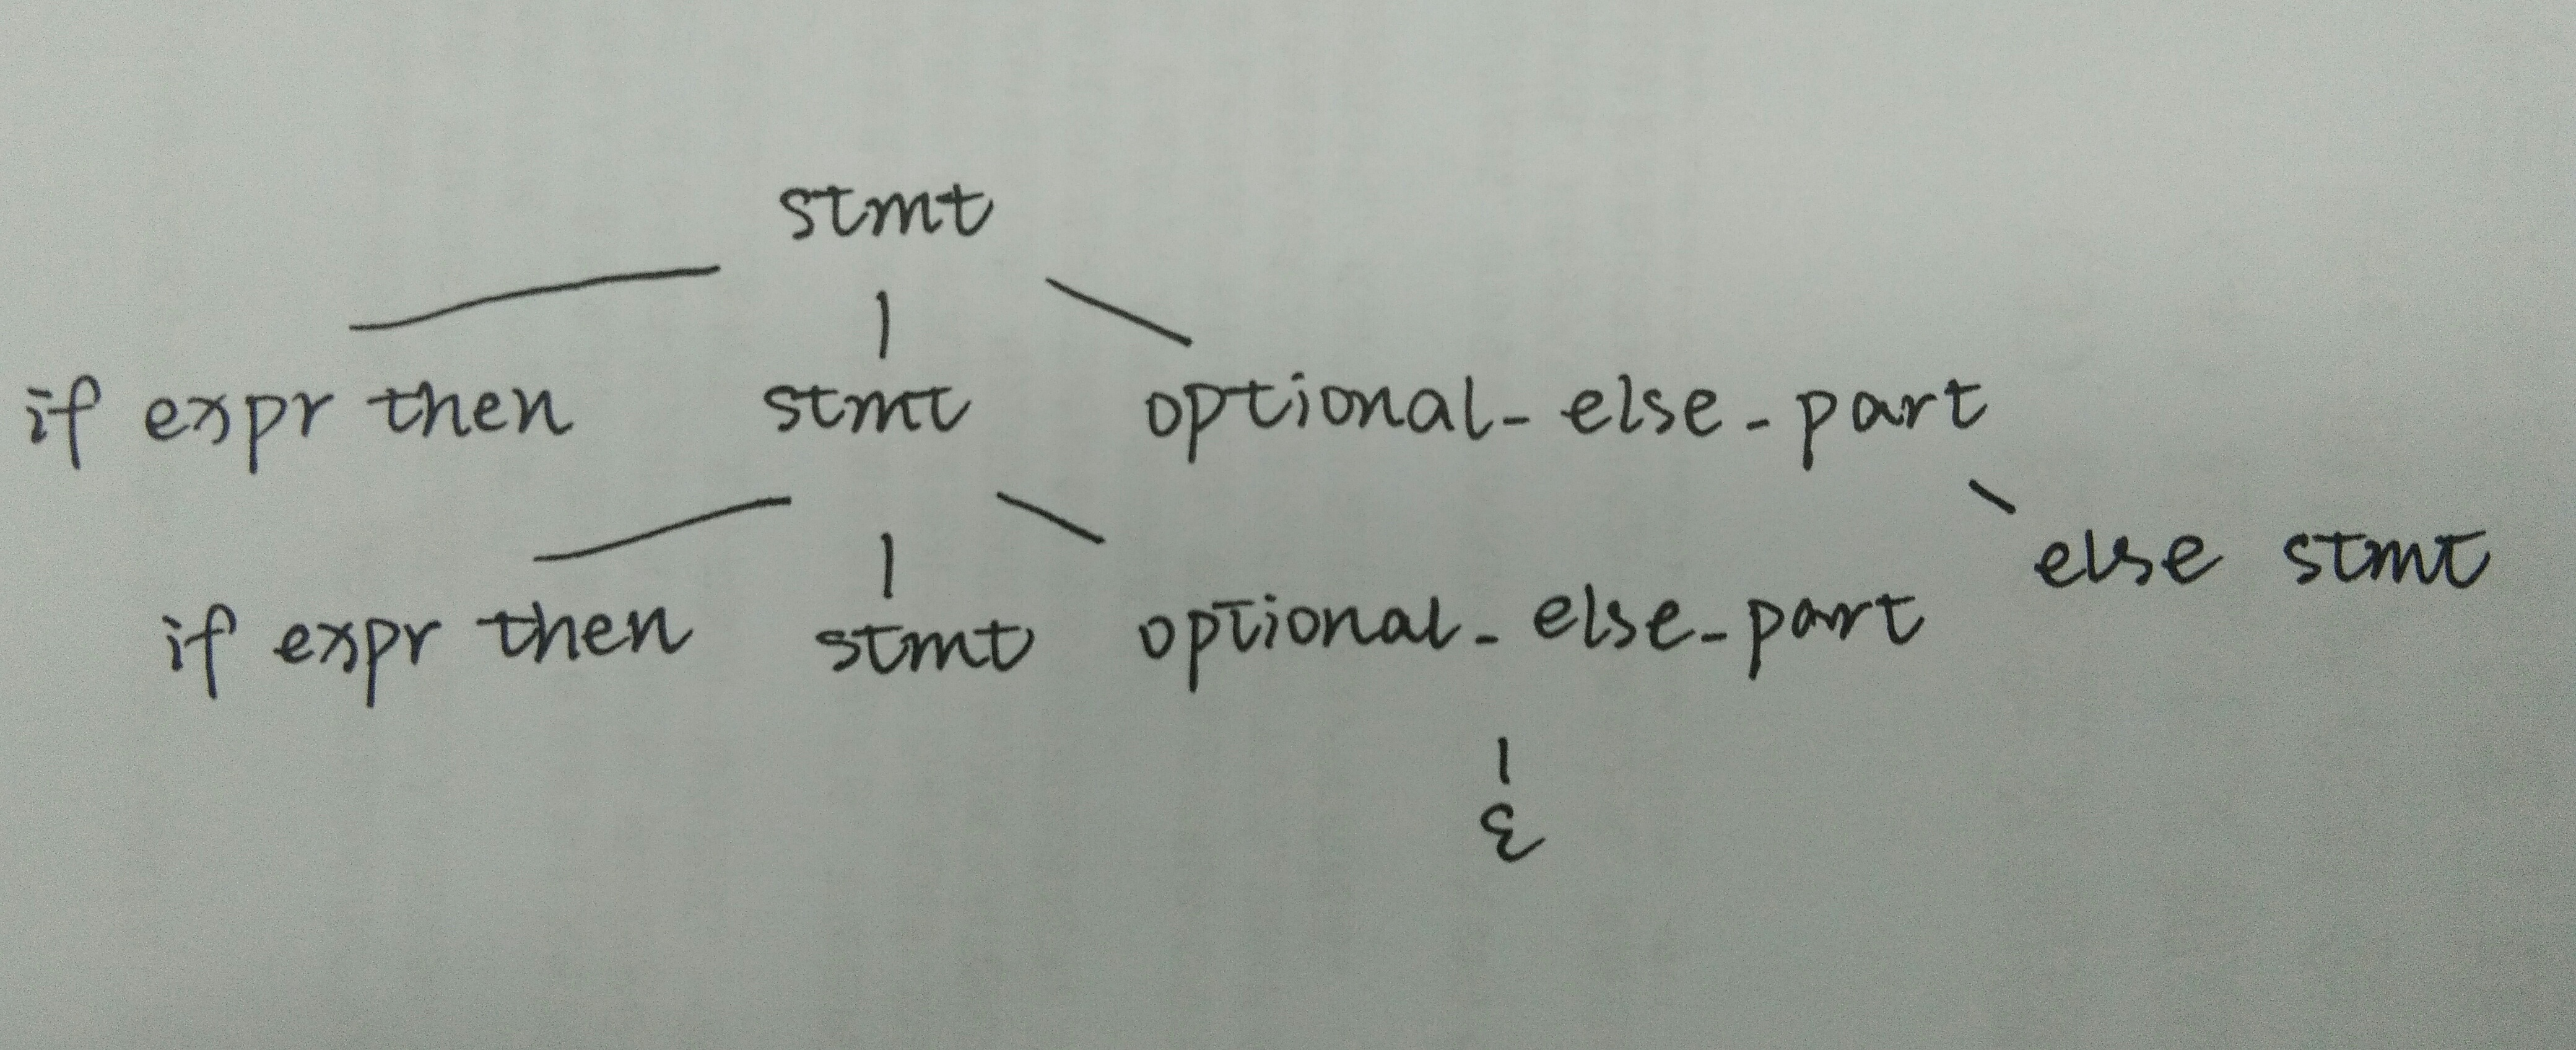
\includegraphics[scale = 0.05]{images/Left_Ambiguity_1.JPG}
			\end{minipage}
			\begin{minipage}{20em}
				\centering
				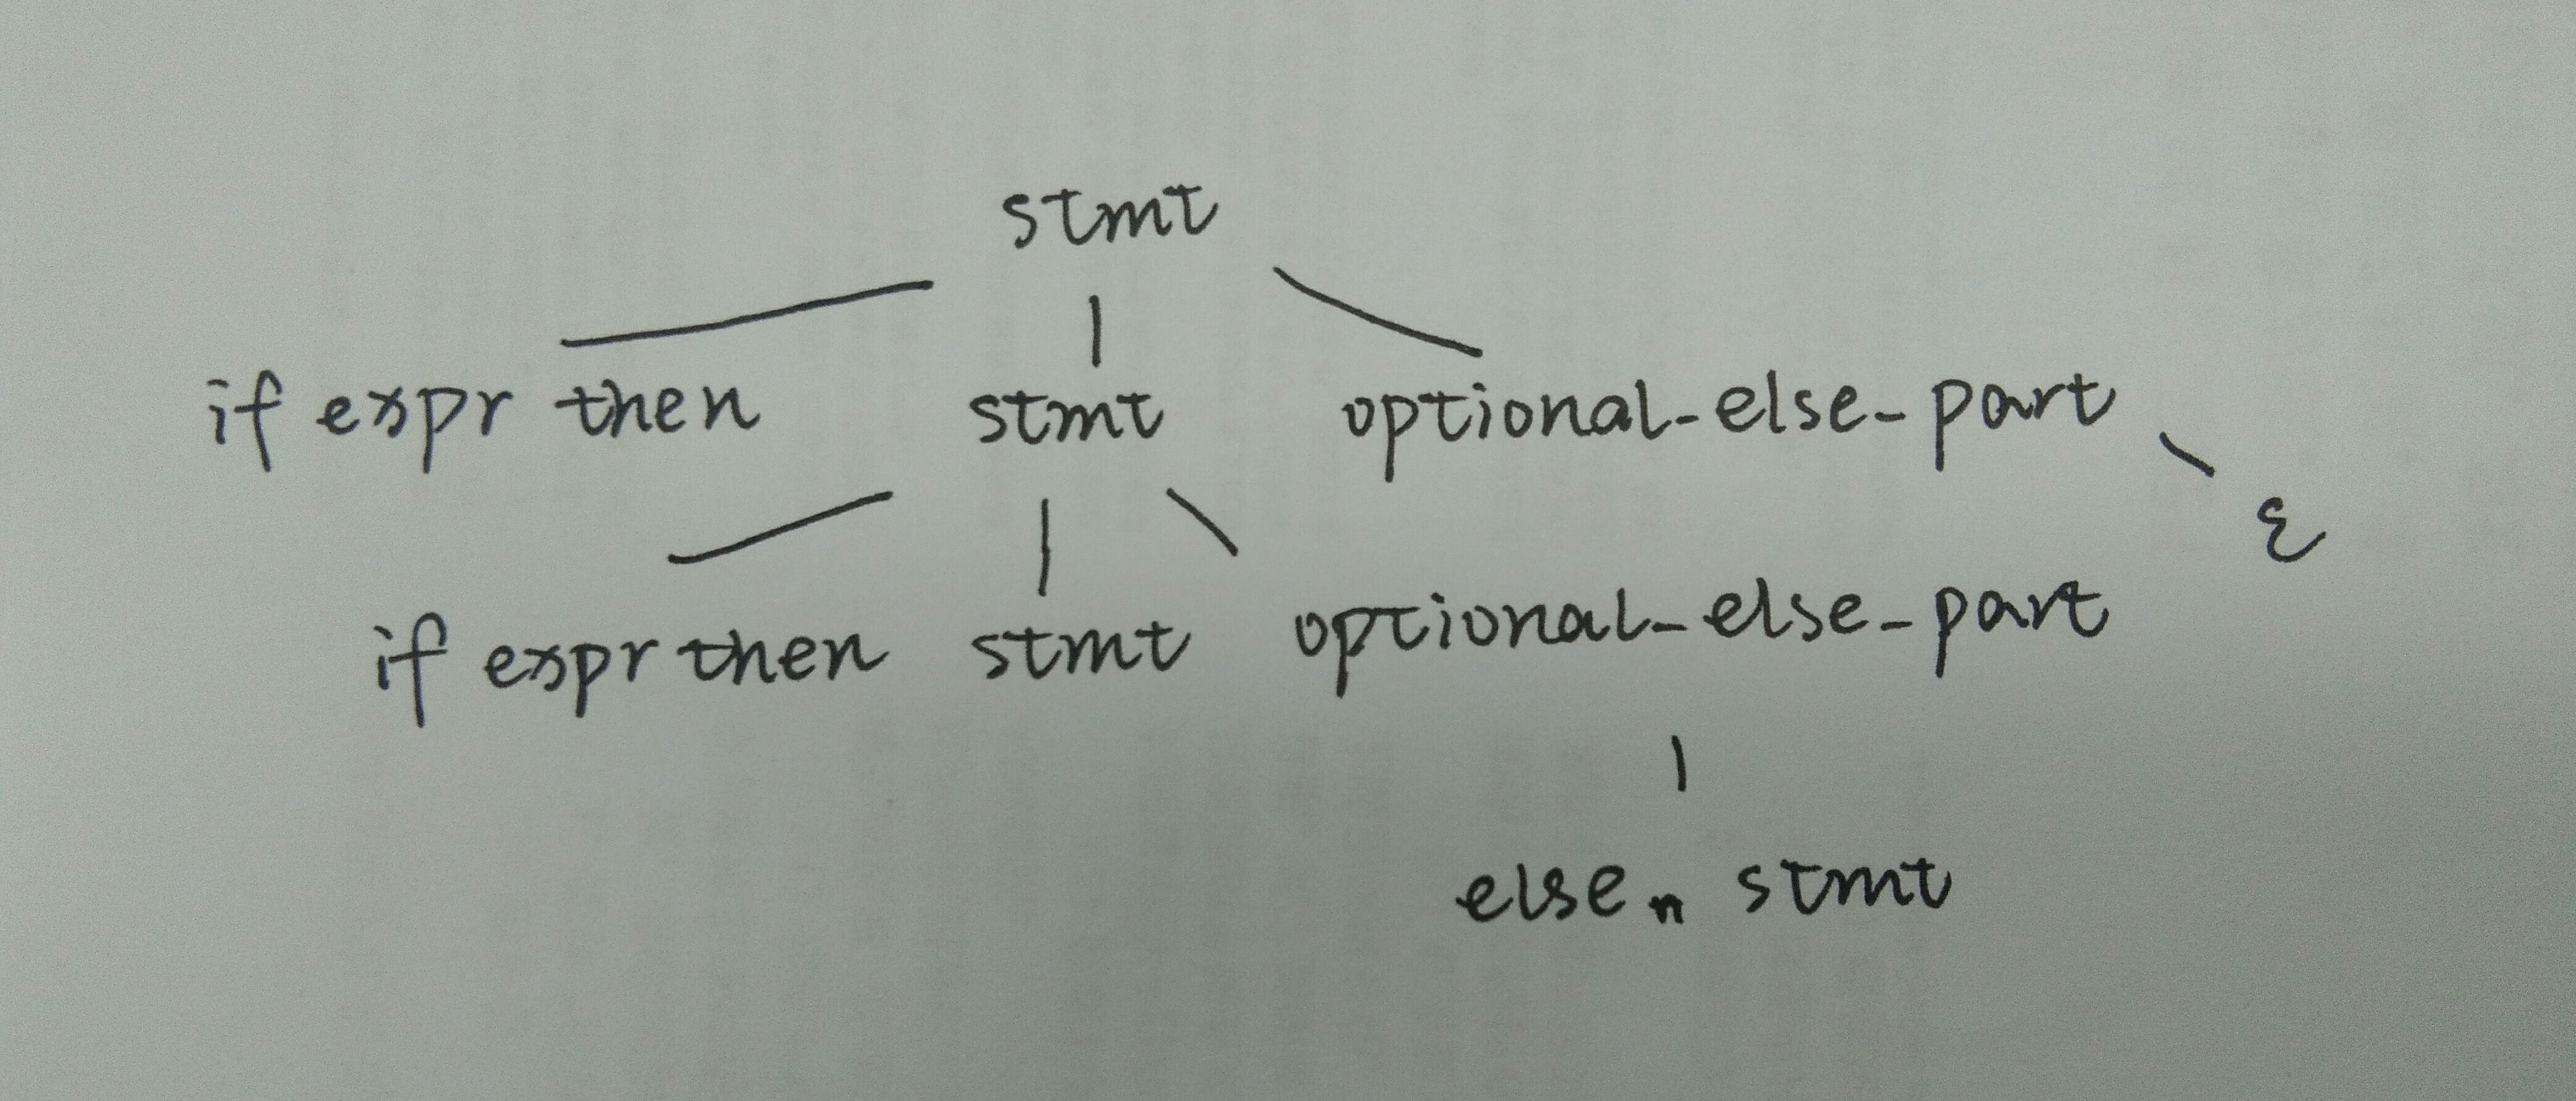
\includegraphics[scale = 0.048]{images/Left_Ambiguity_2.JPG}
			\end{minipage}
		\end{figure}
		\subsection{复杂的回溯代价太高}
		非终结符有可能有多个产生式,由于信息缺失,无法准确预测选择哪一个,考虑到往往需要对多个非终结符进行推导展开,因此尝试的路径可能呈指数级爆炸
	\section{预测分析法}
		Predictive Parsing与递归下降法类似,但是没有若干尝试,没有回溯,采用的通过向前看一些记号来预测需要用到的产生式的方法。此方法接收LL(k)文法,即自左向右读取(left-to-right),最左推导(leftmost derivation),基于对k个记号向前看的推导。在实际应用中,LL(1)用的最广泛。
		\subsection{“第一个”集合和“跟随”集合}
		LL(1)文法中有两个最重要的集合,即FIRST($\alpha$)和FOLLOW($\alpha$)。
		\[FIRST(\alpha)=\{a\mid\alpha\Rightarrow^*a\dots\}\quad\alpha\in V_N,a\in V_T\]
		即,可以从$\alpha$推导出的句型的首部词的集合
		\[FOLLOW(A)=\{a\mid S\Rightarrow^*\dots Aa\dots\}\quad\alpha\in V_N,a\in V_T\]
		即,可能在推导过程中紧跟在A右边的终结符号的集合
		\begin{figure}[h!]
			\centering
			\begin{minipage}{20em}
				\centering
				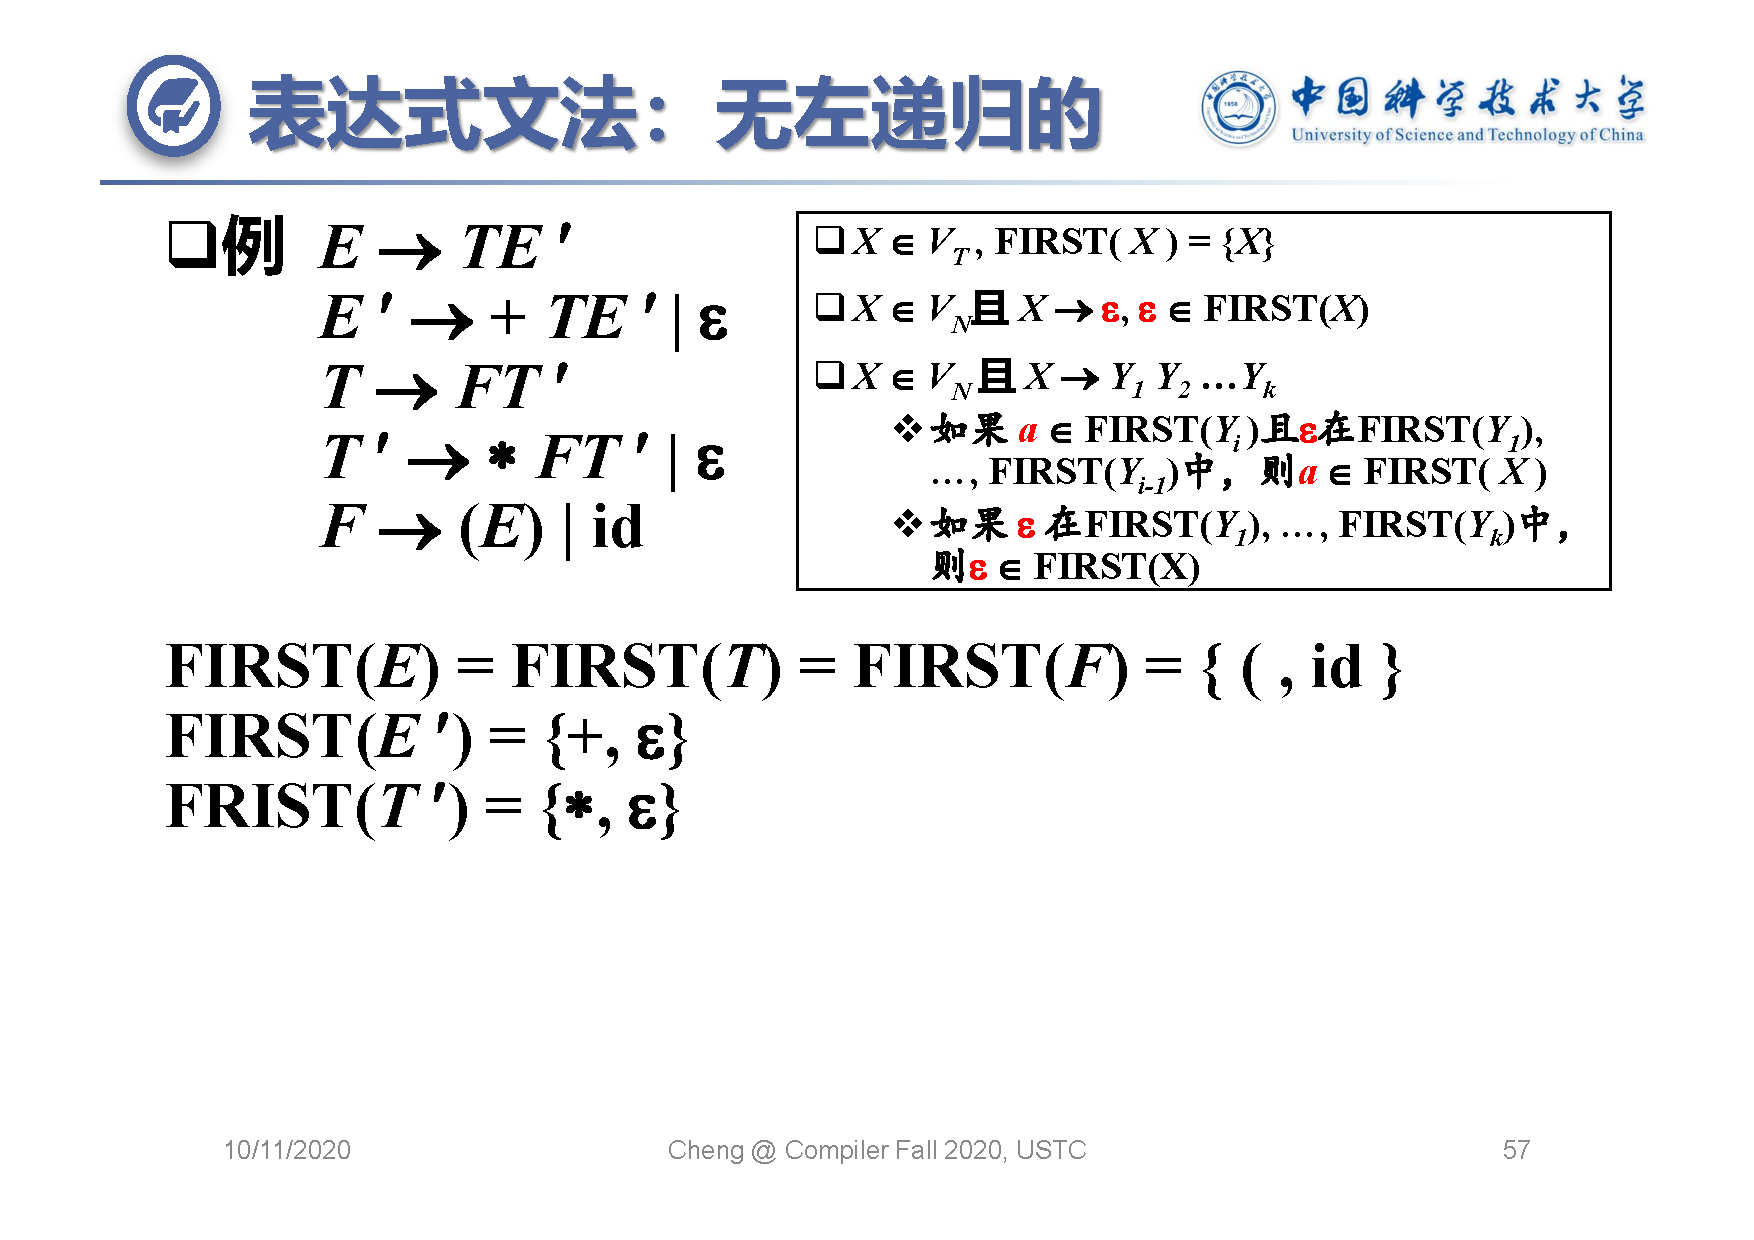
\includegraphics[scale = 0.2]{images/LL1_first.pdf}
				\caption{确定给定推导文法的FIRST集合}
			\end{minipage}
			\begin{minipage}{20em}
				\centering
				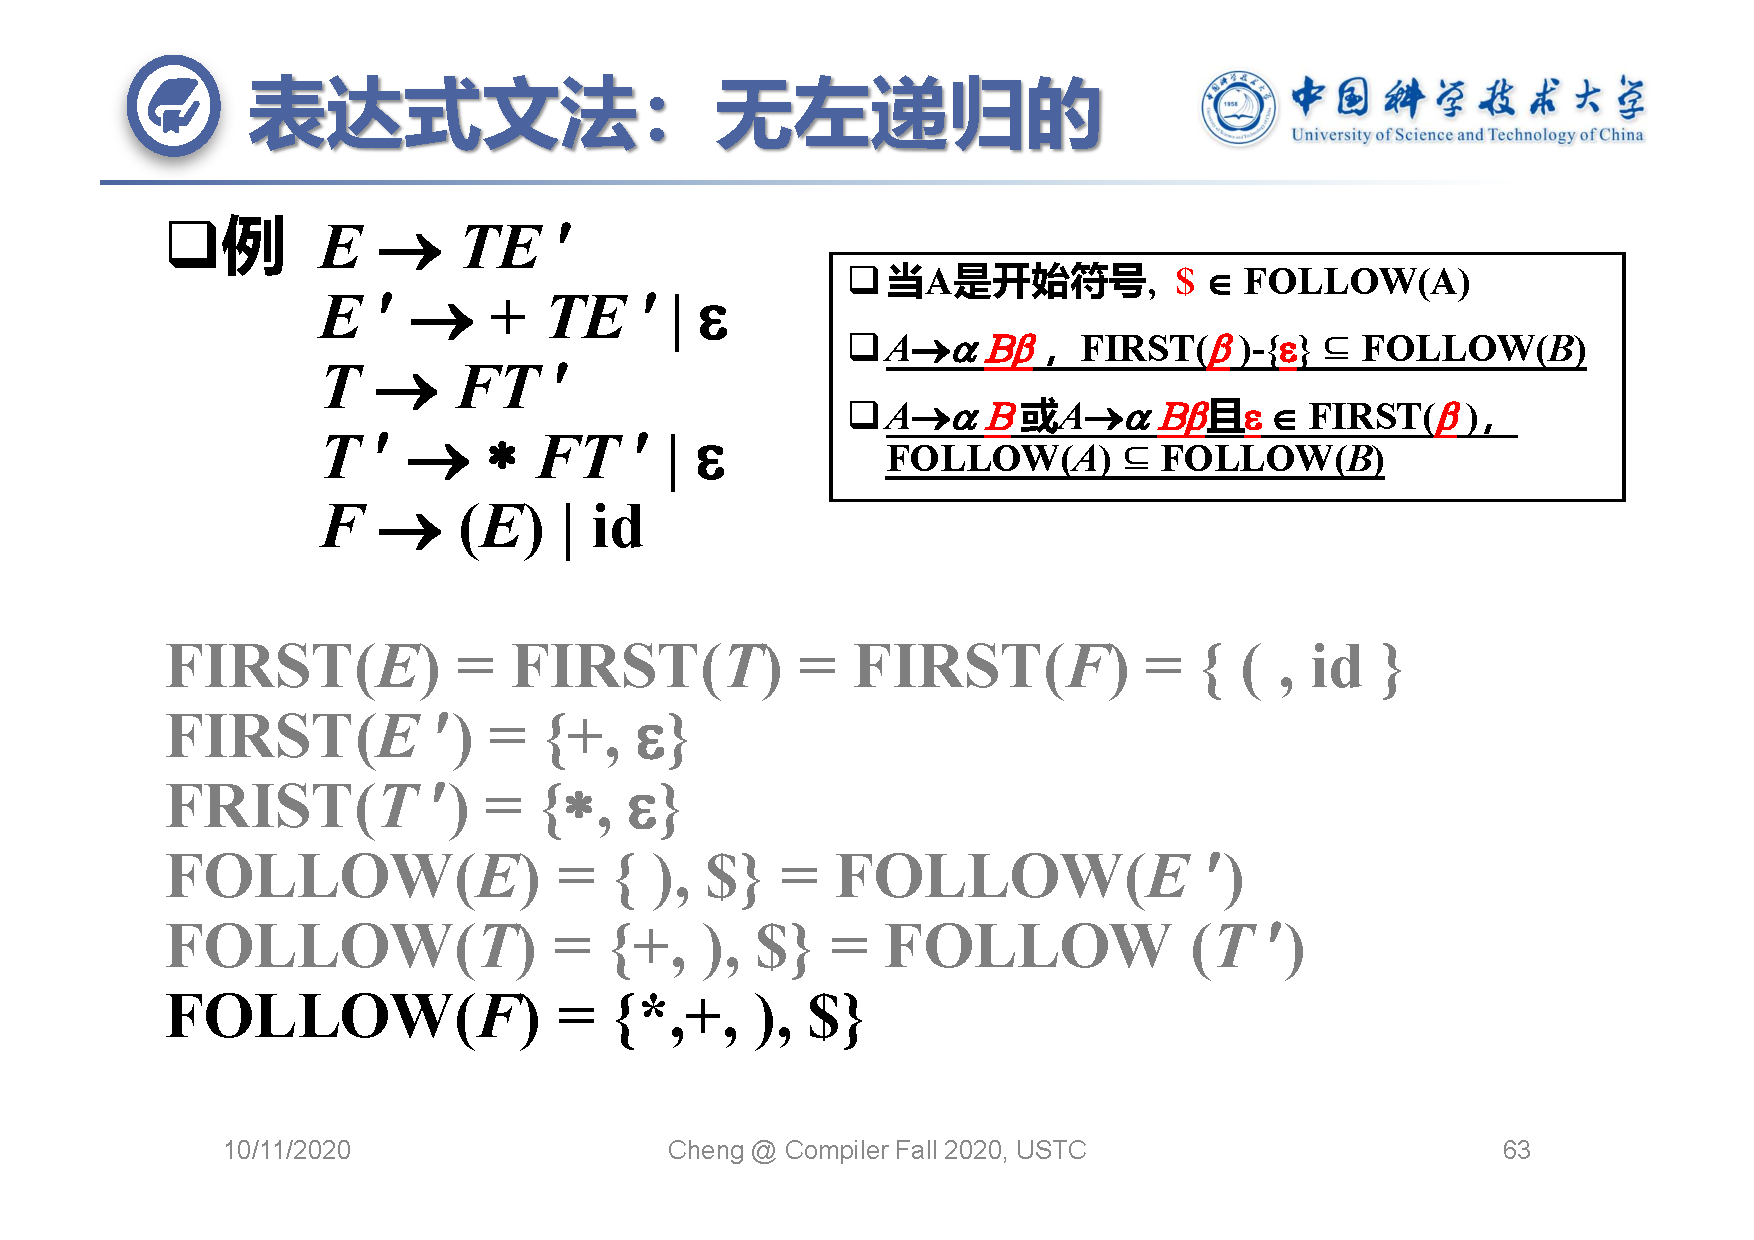
\includegraphics[scale = 0.2]{images/LL1_follow.pdf}
				\caption{确定给定推导文法的FOLLOW集合}
			\end{minipage}
		\end{figure}
		\subsection{LL(1)文法}
		则有LL(1)文法的定义为:对于任何两个产生式$A\to\alpha\mid\beta$都有
		\begin{enumerate}
			\item $FIRST(\alpha)\cap FIRST(\beta)=\varnothing$
			\item 若$\beta\Rightarrow^*\varepsilon$,那么$FOLLOW(A)\cap FIRST(\alpha)=\varnothing$
		\end{enumerate}
		对于第二条,假设$FIRST(A)\cap FIRST(\alpha)=\{a\}$,即
		\[\begin{gathered}
			S\Rightarrow^*\dots Aa\dots\\
			A\Rightarrow^*a\alpha'
		\end{gathered}\]
		又由于$\beta\Rightarrow^*\varepsilon$所以当遇到$Aa$时,既可以用$A\to\alpha$来展开,也可以用$A\to\beta,\beta\Rightarrow^*\varepsilon$来消去A。\par
		LL(1)文法有一些明显的性质,如没有公共左因子(提取左因子)、不是二义的(规则重写)、不含左递归(化为直接左递归,拆分)
		\section{递归下降的预测分析}
		所谓预测分析是指能根据当前的输入符号为非终结符确定采用哪一个选择(预读取k个token)。在这一个部分,主要是要求写出一个预测分析的程序伪代码。伪代码主要是包括两个部分,即$match$函数和对于每一个非终结符的函数。以如下的文法为例:
		\[\begin{gathered}
			type\to simple\mid\uparrow\mathbf{id}\mid\mathbf{array}\ [simple]\ \mathbf{of}\ type\\
			simple\to\mathbf{integer}\mid\mathbf{char}\mid\mathbf{num\ dotdot\ num}
		\end{gathered}\]
		其递归下降预测分析器(伪代码)为(部分):
		\begin{lstlisting}
void match(terminal t)
{
	if (lookahead == t) lookahead = nextToken();
	else error();
}

void type()
{
	if ((lookahead == integer) || (lookahead == char)
		|| (lookahead == num))
		simple();
	else if (lookahead == '\uparrow')
	{
		match ('\uparrow');
		match (id);
	}
	else if (lookahead == array)
	{
		/* code */
	}
	else error();
}
		\end{lstlisting}
		具体来说,就是每一个非终结符$T$,需要构造过程$void T()$,在其中对$T$的产生式右端$\alpha$进行匹配。在匹配的判断中使用$FIRST$集合。匹配之后执行的动作为:非终结符调用他自己的过程,终结符$a$调用$match(a)$
		\subsection{预测分析表}
		对文法的每一个产生式$A\to\alpha$,执行以下两个步骤:
		\begin{enumerate}
			\item 对$FIRST(\alpha)$的每个终结符$A$,把$A\to\alpha$ 加入$M[A, a]$,注意这里的$\alpha$是一个表达式
			\item 对产生式$A\to\alpha$,考虑$FIRST(\alpha)$和$FOLLOW(A)$,如果$\varepsilon$在$FIRST(\alpha)$中,对$FOLLOW(A)$的每个终结符$b$(包括$\$$), 把$A\to\alpha$加入$M[A, b]$
		\end{enumerate}
		值得注意的是,填入表格的$A\to\alpha$是一条推导文法,如$E\to TE'$或者$T'\to\varepsilon$
		注:多重定义条目意味着文法左递归或者是二义的,但是可以通过删除部分条目来消除
	\section{自底向上分析方法}
		\textbf{自左向右读取!}基本方法是归约(右推导的逆过程),用到句柄(可归约串,可能不唯一)的概念,思路是针对输入串,尝试根据产生式规则归约(reduce)到文法的开始符号,是一个比自顶向下更一般化的方法。归约是每一步,特定子串被替换为相匹配的某个产生式左部的非终结符。\par
		对于句柄,句柄是“该句型中和某产生式右部匹配的子串,并且把它归约成该产生式左部的非终结符,代表了最右推导的逆过程的一步”。首先句柄是字串而不一定是一个完整的串,它是在归约过程中某一步产生的句型中的一部分。从另一个方向来看,句柄是对应者自顶向下推导的过程中分析树的非树叶的结点。句柄的右边\textbf{仅包含终结符}(这是因为归约是最右推导的逆过程)。这里“句柄的右边”指的是在这一步规约的句型中,位置在此句柄右边的串。如果文法二义,那么句柄可能不唯一。\par
		比如说,在如下的最右推导(逆过程就是归约)中:
		\[\begin{gathered}
			S\to aABe\\
			A\to Abc\mid b\\
			B\to d\\
			S\Rightarrow_{rm}aABe\Rightarrow_{rm}aAde\Rightarrow_{rm}aAbcde\Rightarrow_{rm}abbcde
		\end{gathered}\]\par
		在句型$aAbcde$中,这一步用于规约的句柄为$Abc$,即“句型中的字串”,同时为产生式$A\to Abc$的右部匹配。
		\subsection{移进(shift)-归约(reduce)分析技术}
		\begin{enumerate}
			\item 两个空间:栈(用来保存已经扫描过的文法符号)、缓冲区(用来保存还未分析的文法符号)
			\item 四个状态:移进(shift,将下一个输入符号放到栈顶,以形成句柄)、归约(reduce,句柄替换为对应的产生式的左部非终结符)、接收(accept,分析成功)、报错(error)
		\end{enumerate}
		移进-归约技术需要解决一些问题,如:
		\begin{enumerate}
			\item 移进-归约冲突(如何决策选择移进(构造句柄)还是归约)
			\item 进行归约时,确定右句型中将要归约的子串(识别句柄)
			\item 归约-归约冲突(进行归约时,如何确定选择哪一个产生式)
		\end{enumerate}
	\section{LR(k)分析技术}
	【回顾】自顶向下和自底向上:\par
	\begin{enumerate}
		\item 自顶向下(Top-down)
		\begin{enumerate}
			\item 针对输入串,从文法的开始符号出发,尝试根据产生式规则推导(derive)出该输入串。
			\item LL(1)文法及非递归预测分析方法
			\item left-to-right scan + leftmost derivation
		\end{enumerate}
		\item 自底向上(Bottom-up)
		\begin{enumerate}
			\item 针对输入串,尝试根据产生式规则归约(reduce)到文法的开始符号。
			\item LR(k)文法及其分析器
			\item left-to-right scan + rightmost derivation
		\end{enumerate}
	\end{enumerate}\par
	一个文法,如果能为他构造出所有条目都唯一都LR分析表,就说他是LR文法。Say,LR语法分析器的关键在于构造LR分析表:\begin{enumerate}
		\item 计算所有可能的状态
		\begin{enumerate}
			\item 每一个状态描述了语法分析过程中所处的位置
			\item 可确定正在分析的产生式集合
			\item 可确定句柄形成的中间步骤
		\end{enumerate}
		\item 明确状态之前的跳转关系
		\item 明确状态与输入之间对应的移进或者归约操作
	\end{enumerate}\par
	LR分析器的格局是二元组,其第一个成分是栈的内容,第二个成分是尚未扫描的输入。活前缀是最右句型的前缀,该前缀不超过最右\textit{句柄}的右端。分析表的转移函数实际上是识别活前缀的DFA,规约函数是对句柄
	\section{SLR}
	文法G的LR(0)项目(简称项目)是在其右部的某个地方加点,表示分析过程的状态的产生式。点的左边是已经看见(读入)的部分,右边是期待看见的部分。或者说,左边是历史信息,右边是展望信息。\par
		\subsection{产生规则} 为了构造出指定文法的SLR分析表,首先重写此文法:
		\begin{enumerate}[label = \circled{\arabic{*}}]
			\item 增加一个新的开始符号(产生拓广文法),即如果之前文法G的开始符号是S,那么增加开始符号$S'$和产生式$S'\to S$,新增产生式的目的是用来指示分析器什么时候应该停止分析并宣布接收输入
			\item 将多路选择的产生式拆分开,比如$E\to E+T\mid T$拆分成$E\to E+T$和$E\to T$两个产生式,这样对判断状态集有好处
			\item 将所有的产生式编号,从$S'\to S\quad(0)$开始
		\end{enumerate}
		然后从新的开始产生式开始,用下面两条规则构造项目集的闭包:(和书上写的不一样)
		\begin{enumerate}
			\item 由上一个状态转换过来的产生式(点向后移动一个位置)
			\item 如果某一条产生式的点在一个非终结符前面,那么看这个非终结符的所有产生式,并将其初始产生式假如到闭包中
		\end{enumerate}
		解释一下上面的规则:
		\begin{enumerate}[label = \circled{\arabic{*}}]
			\item 我自己定义一个概念叫\textit{初始产生式},意思是点加在产生式右部的最左端。(其实就是书上P76写的非核心项目加上$S'\to\cdot S$,如产生式$E\to E+T$,其初始产生式就是$E\to\cdot\, E+T$
			\item 在生成状态$I_0$时,从拓展文法的开始产生式$S'\to S$的初始产生式$S'\to \cdot S$开始
			\item 状态之间的跳转并不需要对前状态的所有元素(产生式)都满足,只表达一种对于此项目集\textbf{可能的}跳转模式
			\item 跳转状态,意味着接收了某种输入
			\item 点在不同位置的同一产生式视作两个不同的项目,需要单独加进去。比如本来我有一个产生式$E\to TE$,现在在闭包里面有$E\to T\cdot E$,我还要加进去$E\to \cdot TE$
		\end{enumerate}
		\subsection{有效项目}
		如果说$S'\Rightarrow^*\alpha Aw\Rightarrow\alpha\beta_1\beta_2 w$,那么就说项目$A\to\beta_1\beta_2$对活前缀$\alpha\beta_1$是有效的。一个项目对于好几个活前缀都可以是有效的,比如若$\beta_2\neq\varepsilon$则应当移进(继续读取才能规约为$A$);若$\beta_2=\varepsilon$,则已经可以直接归约了。
		\subsection{SLR分析表}
		SLR分析表分为左右两部分,左边是动作(action)表,右边是转移(goto)表。二者的行标分别为终结符加$\$$和非终结符,列标为项目集(状态)。action表分为三种情况:
		\begin{enumerate}
			\item 对于没有读取完的产生式项目(点在右部中间,形如$A\to\alpha\cdot a\beta$,$a$为终结符,$\alpha,\beta$可以为$\varepsilon$),设这个项目所在的状态为$I_i$,读取$a$之后会跳转到$I_j$,即$I_i\stackrel{a}{\to}I_j$,那么就在分析表的第i行第a列填入$s_j$
			\item 对于读取完毕的产生式项目,设这个项目所在的状态为$I_i$,产生式的编号为$j$,那么就在分析表的第i行第a列填入$r_j$,其中a是FOLLOW(A)中的所有元素
			\item 对于包含项目$S'\to S\cdot$的状态$i$,在第i行第$\$$列填入$acc$
		\end{enumerate}
		转移表就是说如果状态i在接收非终结符A之后转移到状态j,那么就在第i行第A列填入j
		\subsection{SLR(1)文法}
		一个上下文无关文法G,通过上述算法构造出SLR语法分析表,且表项中没有移进/归约或 者归约/归约冲突,那么G就是SLR(1)文法。1代表了当看到某个产生式右部时,只需要再向前看1个符号就可决定是否用该式进行归约。通常可以省略1,写作SLR文法。
		\subsection{判定满足SLR文法输入串}
		根据SLR文法分析表,使用“文法符号栈-输入缓冲区-对应行为”三联表的形式,尝试读取并分析输入串,直到ACC或者ERR
	\section{规范的LR分析方法}
	在识别活前缀DFA的状态中,增加信息,可以排除一些不正确的归约操作,故规范的LR分析方法增加了前向搜索符:一个项目$A\to\alpha\cdot\beta$,如果真的用这个产生式进行规约之后,期望看到的符号是a(换句话说,在自底向上分析的过程中,对产生式右部$\alpha\beta$进行规约为$A$之后,在$A$的右边应当出现的符号)。LR(1)项目是一个二元组(SLR中的项,搜索符),形式的定义为$[A\to\alpha\cdot\beta,a]$。当$\beta$不为空的时候,a不起作用,当$\beta$为空的时候,如果下一个输入符号为a,那么将按照$A\to\alpha$进行规约,故有$a$的集合是FOLLOW(A)的子集。\par
	\begin{definition}
		对活前缀有效\par
		称LR(1)项目$[A\to\alpha\cdot\beta,a]$对活前缀$\gamma$有效,当且仅当如下情形:如果存在着推导$S'\Rightarrow^*_{rm}\delta Aw\Rightarrow_{rm}\delta\alpha\beta w$,其中$\gamma=\delta\alpha$,a是w的第一个符号,或者a是\$且w是$\varepsilon$
	\end{definition}
		\subsection{构造LR(1)项目集规范族}
		先声明一个我自己瞎起的名字:产生式左边的叫\textit{左值},右边的都叫\textit{右值}。构造方法和SLR的构造方法类似:
		\begin{enumerate}
			\item 不妨设拓广文法的新开始产生式为$S'\to S$,那么从$S'\to\cdot S,\$$开始
			\item 【扩充闭包】在一个状态(项目集)中,对他现有的每一个项目$[A\to\alpha\cdot B\beta,a]$,进行如下构造:
			\begin{enumerate}
				\item 【左值】考虑点后面的非终结符B
				\item 【右值】对于拓展文法中的所有B在左边的产生式$B\to\gamma$(和SLR考虑的一样)
				\item 【搜索符】考虑$FIRST(\beta a)$中的每一个终结符b,并将$[B\to\cdots\gamma,b]$不重复地加入到状态集合中
			\end{enumerate}
			\item 【找全状态】规则和SLR一样,只是要注意,不仅点的位置不同就不同,搜索符不同也不同
		\end{enumerate}
		回顾一下FIRST集合的确定
		\begin{figure}[h!]
			\centering
			\begin{minipage}{20em}
				\centering
				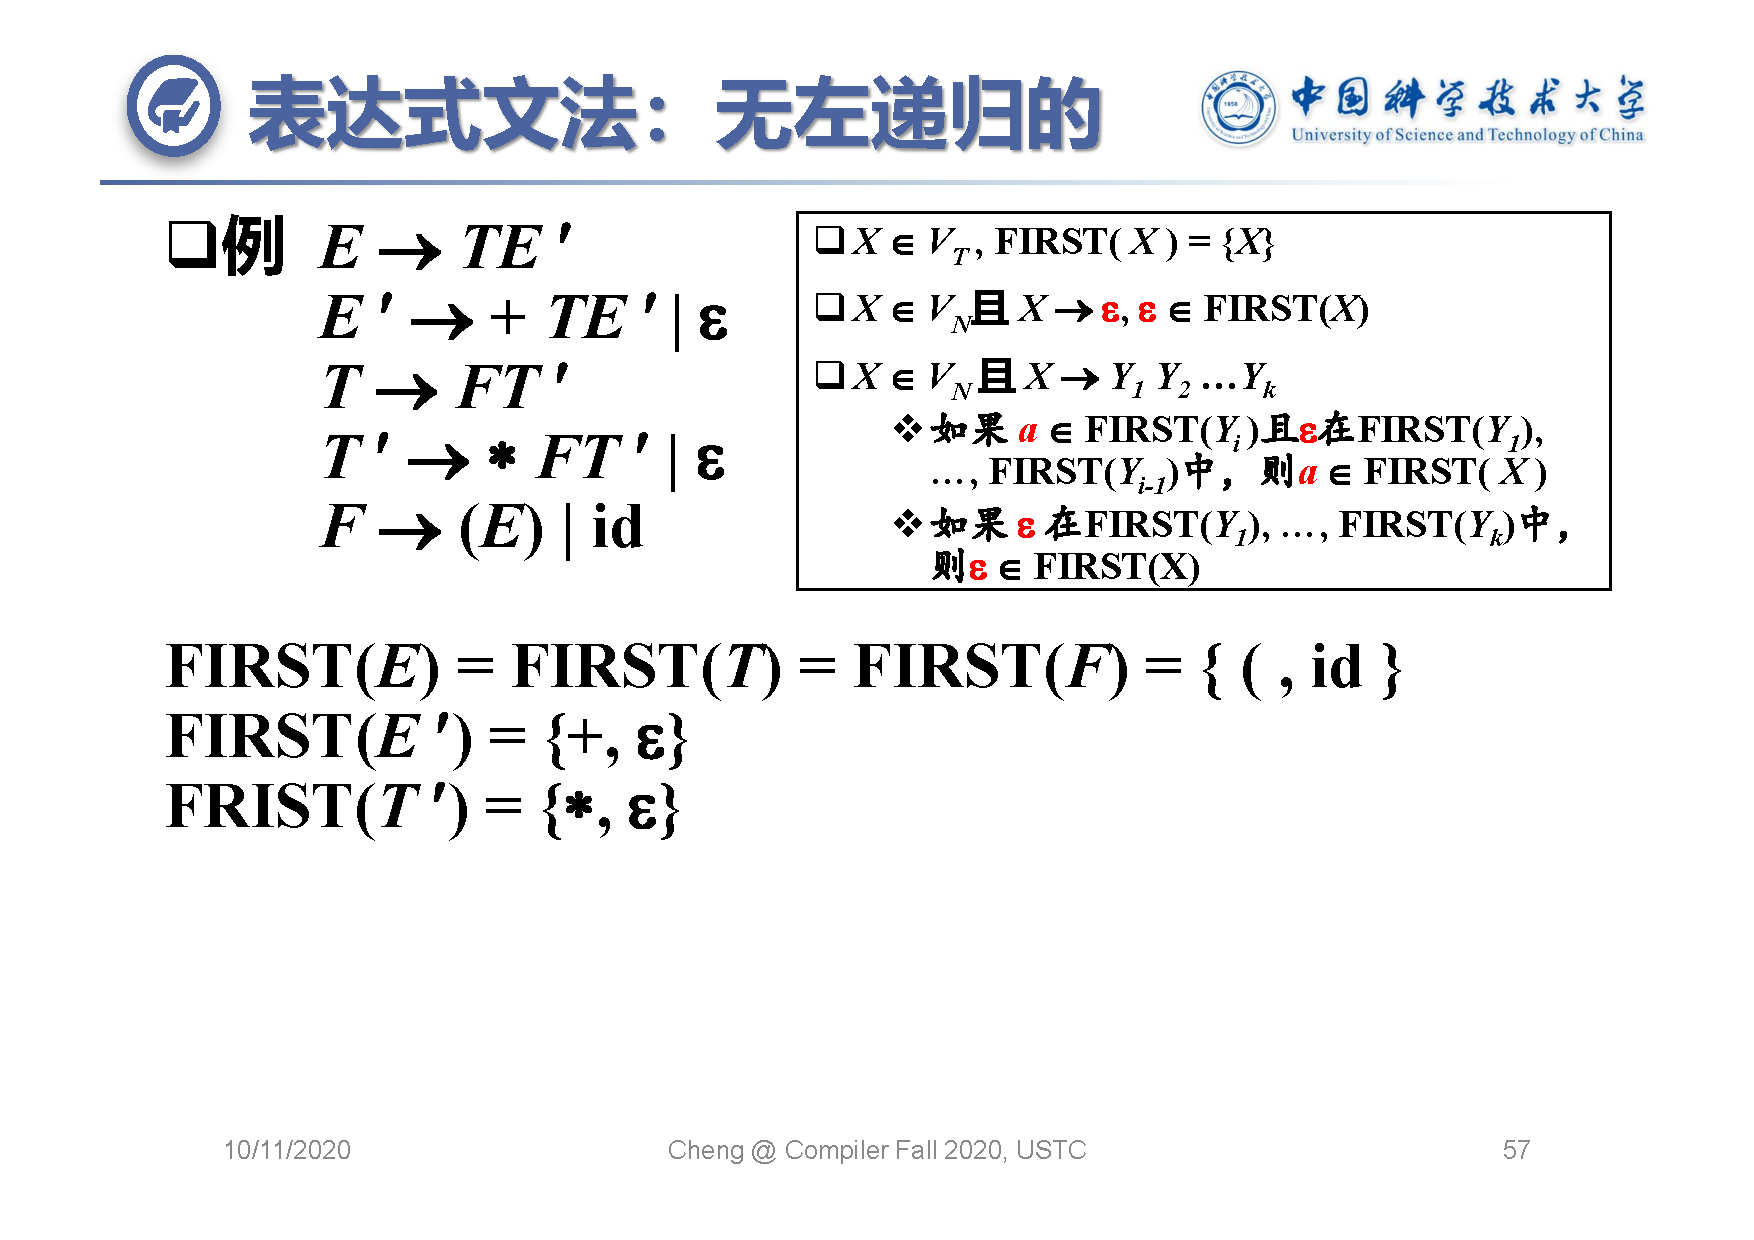
\includegraphics[scale = 0.2]{images/LL1_first.pdf}
				\caption{确定给定推导文法的FIRST集合}
			\end{minipage}
			\begin{minipage}{20em}
				\centering
				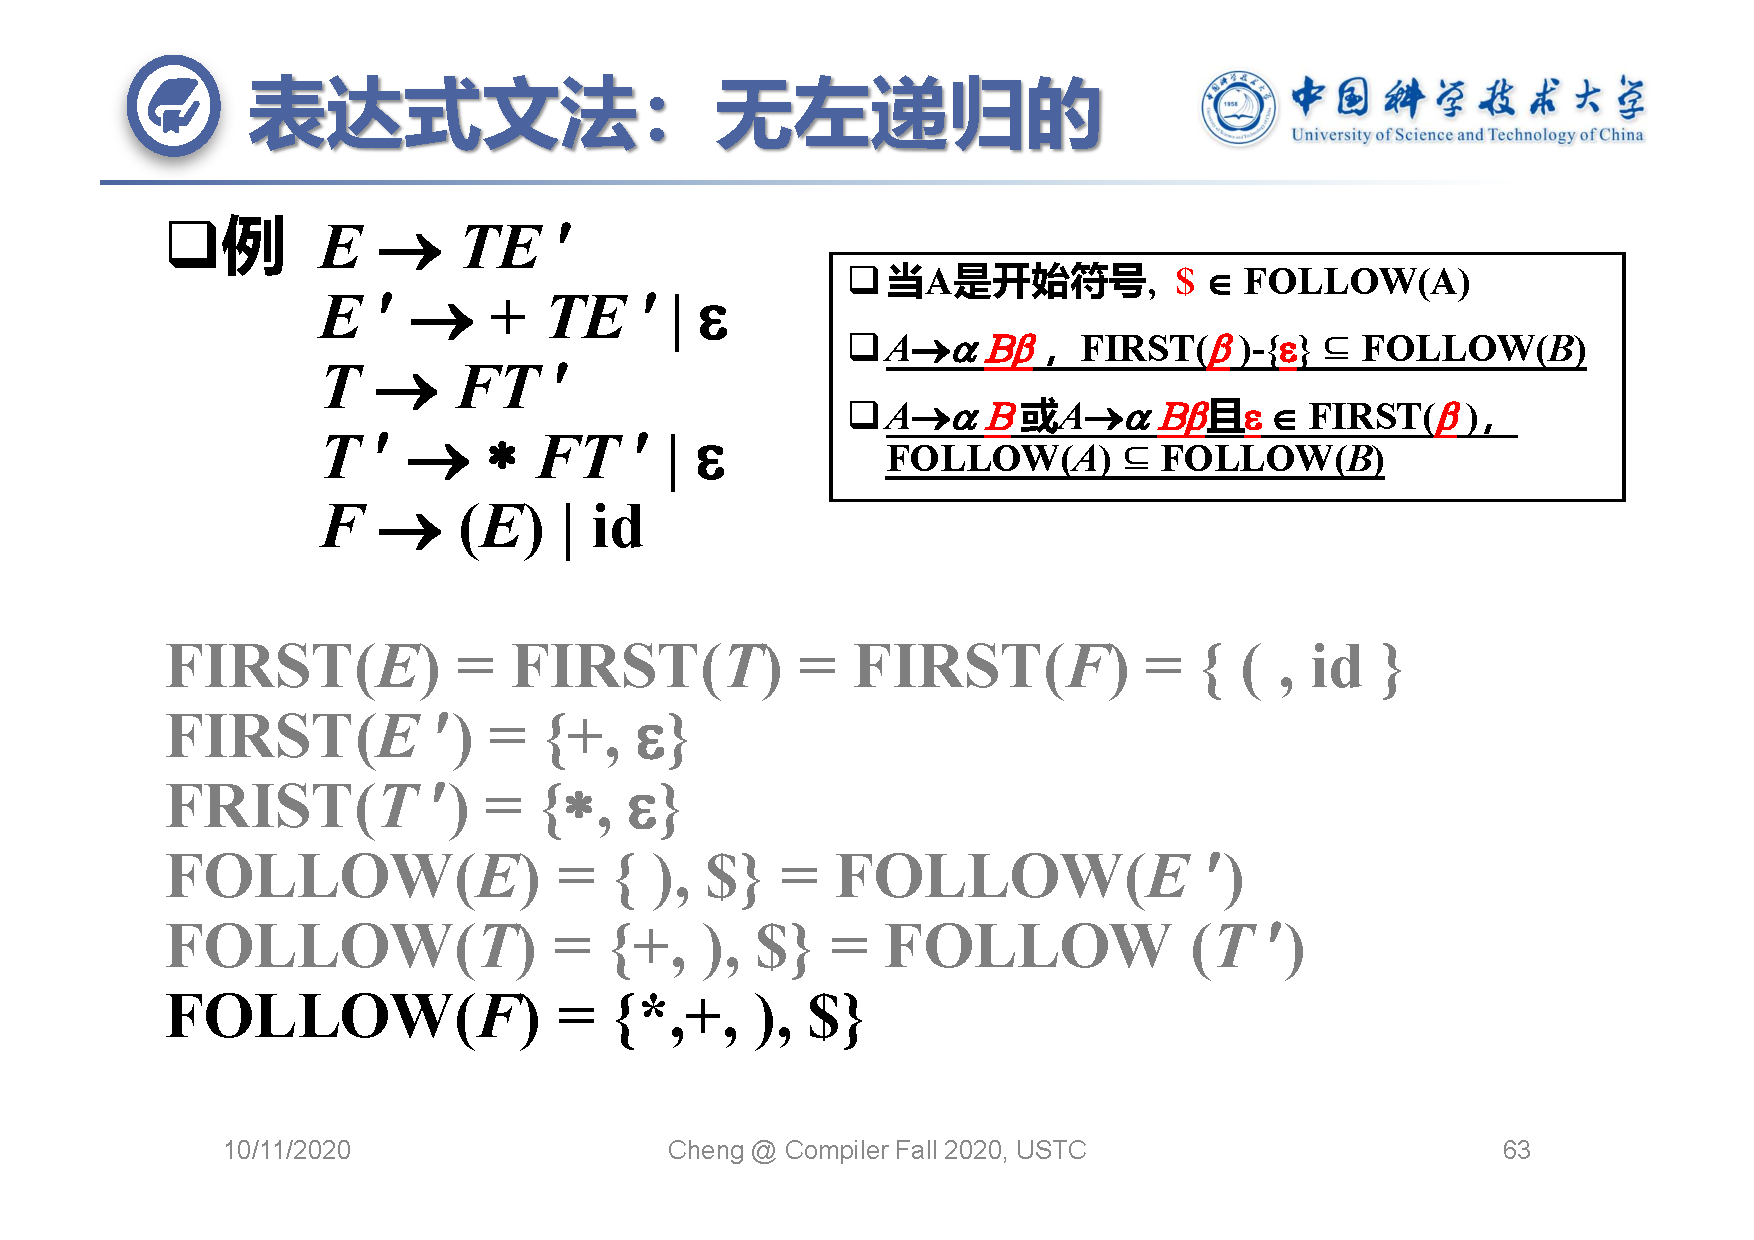
\includegraphics[scale = 0.2]{images/LL1_follow.pdf}
				\caption{确定给定推导文法的FOLLOW集合}
			\end{minipage}
		\end{figure}
		\subsection{构造规范的LR分析表}
		表格形式与SLR类似,但是规则稍有变动:
		\begin{enumerate}
			\item 当点在右值中间时($[A\to\alpha\cdot a\beta,b]$),根据$I_i\stackrel{a}{\to}I_j$,将$s_j$填入i行a列。\textit{注意这种情况下,搜索符b是没有用的。}在这种产生式的形式下,b的唯一用处是在求闭包的时候,求$FIRST(\beta a)$
			\item 当点在右值最右端时,\textbf{不再看FOLLOW(A)},而是对于$I_i$中的所有$[A\to\alpha\cdot,a]$,将$r_j$(j为产生式编号)填入i行a列(其实就是看了FOLLOW的一个子集)
			\item acc和goto不变
		\end{enumerate}
		\subsection{LALR}
		就是在规范LR的基础上合并同心项目集($i.e.$略去搜索符之后他们是相同的集合)。并按照规范LR的规则构造LALR分析表。合并同心项目集可能会引起冲突,但不会引起新的移进-归约冲突

	\chapter{语法制导的翻译}
	这一章开始赋予抽象的符号系统以实际的含义,进入到生成中间代码的阶段。\par
	语法和文法就像数理逻辑中的(语法)和(语义),编译原理的语法是对前面文法分析树在具体程序语言(前提集)上的“赋值”,使得终结符和非终结符有了自己的“属性”。做一组不是很恰当的类比:语法=语法,语义规则=赋值,串=逻辑式,翻译=逻辑式的真假,文法符号=个体变元,属性=指派
	\section{语法制导的定义}
	语法制导(SDD)的定义是带属性和语义规则的上下文无关文法。SDD为CFG中的文法符号设置语义属性,用来表示语法成分对应的语义信息。语法制导翻译是使用上下文无关文法(CFG)来引导对语言的翻译,是一种面向文法的翻译技术。
	\paragraph{如何表示语法信息} 为CFG中的文法符号设置语义属性,用来表示语法成分对应的语义信息
	\paragraph{如何计算语义属性} 文法符号的语义属性值是用与文法符号所在产生式(语法规则)相关联的语义规则来计算的:对于给定的输入串x,构建x的语法分析树,并利用与产生式相关联的语义规则来计算分析树中各结点对应的语义属性值\par
	在语法制导中,用的是基础的上下文无关文法,每一个文法符号有一组属性,每一个文法产生式$A\to\alpha$有一组形式如$b=f(c_1,c_2,\cdots,c_k)$的语义规则,不一定这个产生式中的每一个元素的(每一个)属性都需要写进去。如果b是左值的属性,$c_1,\cdots,c_k$是右值的属性或者左值的其他属性,那么就叫b为综合属性。\textbf{终结符只能有综合属性,属性值无需计算,由词法分析给定}
		\subsection{综合属性和继承属性}
		仅仅使用综合属性地语法制导定义称为S属性定义。但是不是所有情况都这么简单,这时候就会用到继承属性(比如在消除了左递归的文法里面)\par
		总的来说,综合属性将属性自底向上传,而继承属性自上而下传。而对于如下产生式
		\[\begin{gathered}
			T\to FT'\\
			T'\to *FT'_1
		\end{gathered}\]
		在计算T的综合属性$T.syn$时,由于乘法运算符和操作数都隐藏在了$T'$里面,而这个隐藏内容在后续产生式$T'\to*FT'_1$里面,那么就需要将F的属性保存于T'的继承属性里面,传递到下一个“计算周期”,得到结果之后再返回到上一级并传递给T。如下:
		\begin{table}[h!]
			\centering
			\begin{tabular}{cc}
				\toprule
				产生式&语义规则\\
				\midrule
				$T\to FT'$&$T'.inh=F.val,\ T.val=T'.syn$\\
				$T'\to*FT'_1$&$T'_1.inh=T'.inh\times F.val,\ T'.syn=T'_1.syn$\\
				\bottomrule
			\end{tabular}
		\end{table}
		\subsection{注释分析树和属性依赖图}
		根据语法分析,构建出来语法分析树,然后在每一个节点根据其属性值进行计算。当这些属性都是综合属性时,计算可以自底向上地完成。\par
		如果分析树上的一个节点的属性b依赖于某个节点的属性c,那么b的语义规则的计算必须在c之后。这种依赖关系可以用一种称为\textbf{依赖图}的有向图来描述。
		\paragraph{虚拟属性}
		在构造分析树的依赖图之前,先为由过程调用组成的语义规则引入虚拟综合属性$b$,使得每一条规则都能写成$b=f(c_1,c_2,\cdots,c_k)$的形式。在语义分析时,每一个产生式都有一个综合属性(至少在向上返回的时候会用到的)。在后续推理过程中,逐渐(按需)加入继承属性。\par
		属性依赖图的组成是:分析树上的每个结点的每一个属性,都在依赖图上构造一个结点,如果属性b依赖于属性c,那么从c到b连一条有向边。
		\begin{enumerate}
			\item 属性值为点(vertex):分析树中每个标号为X的结点的每个属性a都对应着依赖图中的一个结点
			\item 属性依赖关系为边(edge):如果属性X.a的值依赖于属性Y.b的值,则依赖图中有一条从Y.b的结点指向X.a的结点的有向边
		\end{enumerate}
		\paragraph{属性计算次序}
		由语法制导定义规范的翻译可以准确地按照以下步骤(分析树方法)完成:
		\begin{enumerate}
			\item 根据基础文法构造输入的分析树
			\item 构造属性依赖图
			\item 对依赖图进行拓扑排序,得到语义规则对计算次序
			\item 按这个次序计算属性得到输入串的翻译
		\end{enumerate}
	\section{S属性定义的自下而上计算}
	仅仅使用综合属性的语法制导定义称为S属性的SDD,或S-属性定义、S-SDD。
		\subsection{语法树}
		语法树是分析树的浓缩表示。在语法树中,算符(非终结符)和关键字(终结符)不是作为叶结点,而是作为分支结点。语法树上的内部结点都代表运算,其子节点都是他的运算对象。如同在分析树中那样,在语法树中也可以把属性附加到结点。\par
		语法树的结点可以用有若干指针域的记录来实现。对于算符结点,一个域放运算符,作为结点对象的标记,其余两个域存放只想运算对象的指针。对于基本运算对象结点,一个放\textbf{运算对象类型},一个放他的值。在真正用于翻译时,语法树的结点可能还有其他域来保存其他属性值,或者属性值的指针(比如说,对于产生式$S\to\mathbf{if}\ B\ \mathbf{then}\ S_1\ \mathbf{else}\ S_2$,运算符\textbf{if-then-else}就有4个域(自己和三个运算对象)
		\subsection{S属性的自下而上计算}
		S属性定义的翻译器可以借助LR分析器的生成器来实现,LR可以把文法符号的综合属性放入栈内。\par
		扩展LR的语法分析栈:
		\begin{enumerate}
			\item 在分析栈中使用一个附加的域来存放综合属性值。若支持多个属性,那么可以在栈中存放指针
			\item 每一个栈元素包含状态、文法符号、综合属性三个域。也可以将分析栈看成三个平行的栈,分别是状态栈、文法符号栈、综合属性栈,分开看的理由是,入栈出栈并不完全同步(即有些时候会有某一项不变的情况)
			\item 语义动作将修改为对栈中文法符号属性的计算
		\end{enumerate}\par
		栈操作代码:分为对照的两部分,产生式和代码段。和之前的代码段(对综合属性的赋值及运算)不同,这里由于将正在被分析的结点(们)的属性都入栈了(还维护了一个top指针),现在将这些属性用他们在栈中的位置来表达。注意在这个自底向上的分析中,每一行栈的排布是:产生式“右值”从右向左依次从栈顶向下排,在执行这一步的归约之后pop出去所有的右值,并将左值入栈。\par
		总的来说,采用自底向上分析,例如LR分析,首先给出 S-属性定义,然后,把S-属性定义变成可执行的代码段,放到产生式尾部,这就构成了翻译程序。(注:看一下紫书P118-119的表4.5,前三栏分别为状态栈、文法符号栈、综合属性栈)。
	\section{L属性定义的自上而下计算}
	显然,S属性定义属于L属性定义。
		\subsection{翻译方案}
		语法制导的翻译方案和语法制导定义不同之处是他的语义动作(在此不叫语义规则)放在花括号内,并且可以插入到产生式右部的\textbf{任何地方},即这种表示法动作与分析交错。若$A\to\alpha\{\cdots\}\beta$,那么花括号中语义动作的执行要在$\alpha$的推导结束之后,在$\beta$的推导开始之前。下面是有关继承属性的几个限制:
		\begin{enumerate}
			\item 产生式右部符号的继承属性必须在先于这个符号的动作中计算
			\item 一个动作不能引用该动作右边符号的综合属性
			\item 左值的综合属性要放在右部的末端
			\item 多个继承属性,要考虑次序,避免形成环
		\end{enumerate}


	\chapter{中间代码生成}
	中间表示设计的选择随编译器不同而不同。中间表示可以是一种实际的语言,也可以是编译各阶段共享的内部数据结构。C是一种编程语言,但它经常被当作一种中间形式,这是因为它灵活,能生成高效的机器代码,并且他的编译器到处可用。
	\section{中间语言}
		\paragraph{后缀表示}
		\paragraph{图形表示(有向无环图,即DAG)}
		\paragraph{三地址代码}
		三地址代码是语法树或者DAG的一种线性表示,其中新增加的临时名字对应图的内部结点
		\paragraph{静态单赋值形式,SSA}
	\section{布尔表达式和控制流语句}
		在编程语言中,布尔表达式有两个基本目的,第一是用于计算逻辑值,第二而且更经常的是作为条件表达式,用于控制流语句,如if-then、if-then-else和while-do语句
		\subsection{布尔表达式}
			下面是本节所用的布尔表达式文法:(relop是关系运算符,如$<,>,\le,\ge,==,!=$等)
			\[B\to B\ \mathbf{or}\ B\mid B\ \mathbf{and}\ B\mid\mathbf{not}\ B\mid(B)\mid E\ \mathbf{relop}\ E\mid\mathbf{true}\mid\mathbf{false}\]\par
			实现布尔表达式有两种方法:将真和假数值化,这样布尔表达式的计算就类似于算术表达式的运算;另一种方法就是借助控制流,即\textit{用程序中的位置来表示布尔表达式的值},适用于短路计算的情况。
		\subsection{控制流语句的翻译}
			控制流语句(if-then、if-then-else、while-do、顺序执行)由下面的文法产生(B是布尔表达式):
			\[\begin{aligned}
				S\to
				&\mathbf{if}\ B\ \mathbf{then}\ S_1\\
				&\mid\mathbf{if}\ B\ \mathbf{then}\ S_1\ \mathbf{else}\ S_2\\
				&\mid\mathbf{while}\ B\ \mathbf{do}\ S_1\\
				&\mid S_1;S_2
			\end{aligned}\]\par
			这四种语句对应的代码栈如下图所示,这几个图所示的三地址代码的结构可以帮助理解next的跳转。需要注意的是,$S.next$并没有被显式地画出来,而是作为(已知的)整个语句的出口,在后面的代码生成语法制导定义中被赋值给某些(语句块的)出口
			\begin{figure}[ht!]
				\centering
				\begin{minipage}{40em}
					\centering
					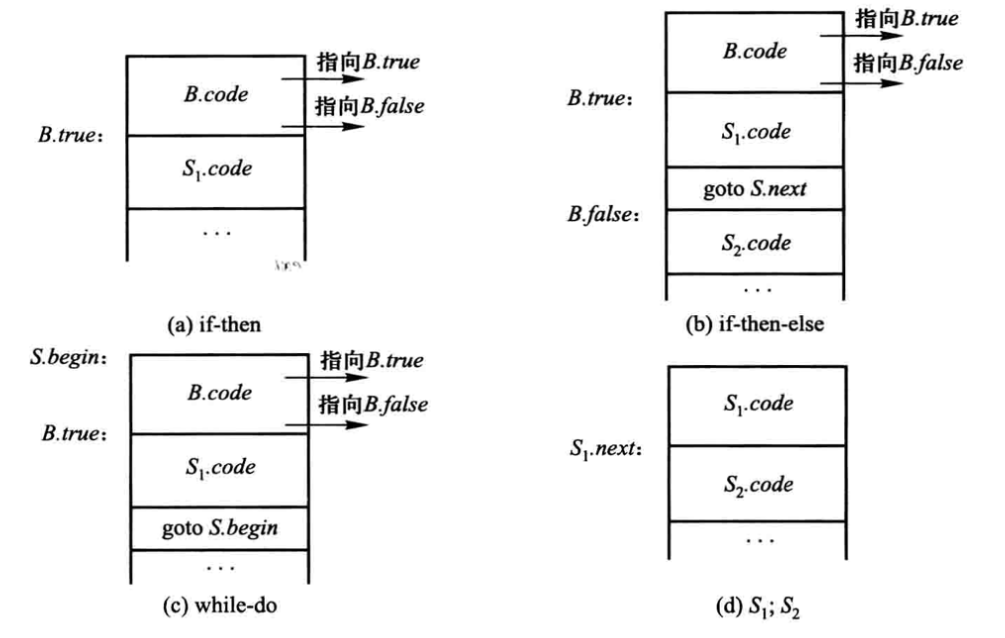
\includegraphics[scale = 0.4]{images/Bool_Expression_If_Code.png}
					\caption{if-then,if-then-else,while-do和顺序语句的代码(栈)}
				\end{minipage}
			\end{figure}
		\subsection{if语句中间代码生成的SDD}
			姑且命名语句$S\to\mathbf{if}\ B\ \mathbf{then}\ S_1$为产生式$\gamma$。\par
			这个“产生式”的每一个“非终结符”($S,B,S_1$)都是一段代码,即他们的综合属性$S.code,\ etc$。每一个代码段都要有一个或多个“出口”,也就是说在执行结束这一段代码之后程序应当去往何方。这些“出口”用“非终结符”的继承属性来表示。可以调用$newlabel()$来产生新标号,新标号是跳转到这个产生式内部的时候,用(实际上是另一个非终结符的$.begin$的位置的)一个内部入口,而不是(将整个产生式封装起来看,放在“左值”的$.next$属性中的)一个总的出口,来对这个$.next$属性赋值。即:
			\begin{enumerate}
				\item 标号指向内部的三地址代码时需要调用$newlabel()$
				\item 标号指向外部的三地址代码时从$S$继承
			\end{enumerate}\par
			语义规则:
			\[\begin{gathered}
				B.true=newlabel()\\
				B.false=S.next\\
				S_1.next=S.next\\
				S.code=B.code\parallel gen(B.true,':')\parallel S_1.code
			\end{gathered}\]
		\subsection{带有else的语句的中间代码生成}
			考虑带来else的语句$S\to\mathbf{if}\ B\ \mathbf{then}\ S_1\ \mathbf{else}\ S_2$。\par
			对布尔表达式B,用两个标号$B.true$和$B.false$分别表示B为真和为假时控制流应该转向的标号,这两个属性由B的上下文决定。注意在$S_1.code$的后面由$\mathrm{goto}\ S.next$,这条指令是需要的,因为$S_1$执行结束意味着$S$执行结束,并且当$S_1$是赋值语句的时候肯定会执行这条指令

\end{document}
